\documentclass[review,3p,twocolumn,times]{elsarticle}

\usepackage{lineno,hyperref}
\modulolinenumbers[5]

\usepackage{graphicx}
\usepackage{floatrow}
\floatsetup[table]{capposition=top}
\newfloatcommand{capbtabbox}{table}[][\FBwidth]
\usepackage{subfigure}
\graphicspath{{Figures/}}
\usepackage[T1]{fontenc} % optional
\usepackage{amsmath}
\usepackage{epstopdf}
\usepackage{indentfirst}
\usepackage{amsmath}
\usepackage{fancyhdr}
\usepackage{algorithm}
\usepackage{algorithmic}
%\usepackage{multicol}
\usepackage{diagbox}[2011/11/22]
\usepackage{enumerate}
\newcommand{\tabincell}[2]{\begin{tabular}{@{}#1@{}}#2\end{tabular}}
%\newcommand{\upcite}[1]{\textsuperscript{\cite{#1}}}
\usepackage{multirow}
\usepackage{multirow}
\usepackage[normalem]{ulem}
\usepackage{comment}
\usepackage{threeparttable}
\usepackage{mathrsfs,amsfonts,amssymb}
\useunder{\uline}{\ul}{}
\usepackage{geometry}
\usepackage{rotating}
\floatname{algorithm}{Procedure}
\geometry{top=2.5cm,bottom=3cm}
\newcommand{\upcite}[1]{\textsuperscript{\cite{#1}}}

\usepackage{supertabular}
\usepackage{array}
\usepackage{booktabs} %调整表格线与上下内容的间隔
\usepackage{amsmath} 
\usepackage{amssymb}
\usepackage{url}
\renewcommand{\baselinestretch}{1.2}

\journal{Pattern Recognition}

%%%%%%%%%%%%%%%%%%%%%%%
%% Elsevier bibliography styles
%%%%%%%%%%%%%%%%%%%%%%%
%% To change the style, put a % in front of the second line of the current style and
%% remove the % from the second line of the style you would like to use.
%%%%%%%%%%%%%%%%%%%%%%%

%% Numbered
%\bibliographystyle{model1-num-names}

%% Numbered without titles
%\bibliographystyle{model1a-num-names}

%% Harvard
%\bibliographystyle{model2-names.bst}\biboptions{authoryear}

%% Vancouver numbered
%\usepackage{numcompress}\bibliographystyle{model3-num-names}

%% Vancouver name/year
%\usepackage{numcompress}\bibliographystyle{model4-names}\biboptions{authoryear}

%% APA style
%\bibliographystyle{model5-names}\biboptions{authoryear}

%% AMA style
%\usepackage{numcompress}\bibliographystyle{model6-num-names}

%% `Elsevier LaTeX' style
\bibliographystyle{elsarticle-num}
%%%%%%%%%%%%%%%%%%%%%%%

\begin{document}

\begin{frontmatter}

\title{Ensemble of ML-KNN for Classification Algorithm Recommendation}
%\tnotetext[mytitlenote]{Fully documented templates are available in the elsarticle package on \href{http://www.ctan.org/tex-archive/macros/latex/contrib/elsarticle}{CTAN}.}

%% Group authors per affiliation:
%\author{Elsevier\fnref{myfootnote}}
%\address{Radarweg 29, Amsterdam}
%\fntext[myfootnote]{Since 1880.}

%% or include affiliations in footnotes:
\author[xjtuaddress]{Xiaoyan Zhu\corref{correspondingauthor}}
\cortext[correspondingauthor]{Corresponding author}
\ead{zhu.xy@xjtu.edu.cn}

\author[xjtuaddress]{Chenzhen Ying}

\author[xjtuaddress]{Jiayin~Wang}

\author[michaddress]{Guangtao Wang}


\address[xjtuaddress]{School of Electronic and Information Engineering,
	Xi$'$an Jiaotong University, Xi$'$an, China}
%\address[michaddress]{Department of Computational Medicine and Bioinformatics, University of Michigan, Ann Arbor, USA}
\address[michaddress]{JD AI Research, Mountain View, California}
%\author[mymainaddress,mysecondaryaddress]{Elsevier Inc}
%\ead[url]{www.elsevier.com}
%
%\author[mysecondaryaddress]{Global Customer Service\corref{mycorrespondingauthor}}
%\cortext[mycorrespondingauthor]{Corresponding author}
%\ead{support@elsevier.com}
%
%\address[mymainaddress]{1600 John F Kennedy Boulevard, Philadelphia}
%\address[mysecondaryaddress]{360 Park Avenue South, New York}

\begin{abstract}
 With mountains of classification algorithms proposed in the literature, the study on how to pick up suitable classifier(s) for a given problem is important and practical. Existing methods rely on single learner built on one type of meta feature or a simple combination of several types to tackle this problem. In this paper, we observe that a given classification problem can be characterized in terms of different viewpoints, and various sets of meta-features recognized from the diverse viewpoints would be complementary to each other. We propose a two-layer classification algorithm recommendation method called \emph{EML} (Ensemble of \emph{ML-KNN} for classification algorithm recommendation) to leverage such diversity and complementarity of different sets of meta-features. One key benefit of the proposed ensemble learner is that it constructs multiple base single learners together in a unified framework, and is able to improve the generalization ability of the predictive recommendation model. Moreover, it can automatically recommend different but proper number of appropriate algorithms for different dataset, rather than specify a fixed number of appropriate algorithm(s) as does by \emph{ML-KNN} based and \emph{SLP} (Single link prediction) based method. Experimental results on 183 public datasets show the effectiveness of the \emph{EML} method compared to the \emph{SLP} based and \emph{ML-KNN} based method.
\end{abstract}

\begin{keyword}
 Classification algorithm \sep Recommendation method \sep Ensemble learning 
%\texttt{elsarticle.cls}\sep \LaTeX\sep Elsevier \sep template
%\MSC[2010] 00-01\sep  99-00
\end{keyword}

\end{frontmatter}

\linenumbers

\section{Introduction}
\label{sec:introduction}

Classification is one of the most important problem in data mining and has been widely studied on. There are a large variety of classification algorithms proposed in literature, such as tree based (e.g., ID3\upcite{quinlan1979discovering}, C4.5\upcite{Quinlan1993Programs}, and CART\upcite{breiman1984classification}), probability based (e.g., Naive Bayes\upcite{Moore2005Internet} and AODE\upcite{webb2005not}), and rule based (e.g., OneR\upcite{holte1993very} and Ripper\upcite{Cohen1995Fast}). 

However, both the "No Free Lunch" theory\upcite{Wolpert2002The} and experimental results\upcite{Ali2006On,Brazdil2000A} have demonstrated that there is no specific classification algorithm applicable to all classification problems, namely all classification datasets. Thus, "How to select the appropriate classification algorithm(s) for a given dataset" is a big challenge, especially for non expert.

Studies have showed that the appropriate algorithms vary with different datasets, and the performance of an algorithm is closely associated with the characteristics of the dataset\upcite{song2012automatic}. Therefore, the key up to the challenge is to explore the relationship between the characteristics of the datasets and the performance of the candidate algorithms, and then construct a model to recommend appropriate algorithm(s) for a new dataset. This is a hot spot called algorithm recommendation in the field of data mining, which has drawn the attention of many researchers \upcite{Chekina2012Meta,Smith2009Cross,Brazdil:2008:MAD:1507541,Aha1992Generalizing,Wang2015An,Roy2017Meta,Smith2001Modelling,Smith2002Matching,Kalousis2004On,Gore2013Dynamic,Ali2017Accurate}.

Generally, researchers\upcite{Chekina2012Meta,Brazdil1994Characterizing,Gama1995Characterization,Smith2001Modelling,Smith2002Matching,Brazdil2003Ranking,Kalousis2004On} view classification algorithm recommendation as a meta-learning problem, where the meta-features are the characteristics of a dataset and the meta-target represents the relative performance of candidate algorithms on the dataset. 

Formally, the classification algorithm recommendation problem can be viewed as a learning problem that can be solved in two steps: 1) searching for a function $f: \mathcal{X} \mapsto \mathcal{Y}$, where $ \mathcal{X}=\mathbb{R}^p$ is the meta-feature space with $p$ meta-features and $\mathcal{Y}=\{y_1,y_2,...,y_q\}$ is the meta-target space with $q$ candidate algorithms; 2) recommending appropriate algorithms $Y_{new} \subseteq \mathcal{Y}$ for a new dataset $d_{new}$ according to $f(x_{new})$, where $x_{new} \in \mathcal{X}$ is the meta-features of $d_{new}$.

There are three different representations of meta target $Y$ that have been commonly used in literature, including single-label based, ranking based and multi-label based. With different representations of meta target, different methods can be used to solve the classification algorithm recommendation problem. For single-label based meta target, where $Y=y, y\in\mathcal{Y}$, single label learning methods can be utilized to recommend a single algorithm that achieves the best performance \upcite{Ali2006On,Brazdil1994Characterizing,Lee2013Automatic,Gore2013Dynamic}. For ranking based meta target, where $Y=\{y'_1,y'_2, ..., y'_q|y'_i\in\mathcal{Y} \& y'_i>y'_j, i<j\}$\footnote{Here, $y'_i>y'_j$ means performance of $y'_i$ is better than that of $y'_j$}, ranking learning algorithms \upcite{Brazdil2000A,Brazdil2003Ranking} or regression algorithms \upcite{Bensusan2001Estimating,Reif2014Automatic,Balte2015Algorithm} can be adopted to recommend a ranked list of the candidate algorithms according to their predictive performance.

Wang et al.\upcite{Wang2014A} pointed out and demonstrated that classification algorithm recommendation was closer to a multi-label learning problem. They took all the algorithms that performs statistically equivalent to the best algorithm as appropriate algorithms. Their meta-target $Y\subseteq\mathcal{Y}$ was in multi-label form with all the appropriate algorithms. \emph{ML-KNN}\upcite{Zhang2007A} was used as the multi-label learning method to recommend the top $r$ algorithms for a dataset, where value of $r$ needed to be specified in advance. Their empirical study validated the effectiveness of the \emph{ML-KNN} based classification algorithm recommendation method compared to single-label based and ranking based methods. % The \emph{ML-KNN} based method makes recommendation by taking only neighbors of the datasets into consideration, ignoring the impact of other datasets. 

Zhu et al.\upcite{Zhu2018A} applied single link prediction based method to recommend appropriate algorithms. It achieved better performance than the \emph{ML-KNN} based method because it took the impact of more datasets into consideration, rather than only the neighbors of the given dataset. Nevertheless, performance of the \emph{SLP} based method depends on only one learner, which affects its recommendation performance and leaves room for improvement.

In addition, in the \emph{SLP} based method, the number of the recommended algorithms needs to be specified in advance. But this number varies with different datasets. Wang et al.\upcite{Wang2014A} had shown that when taking 13 algorithms into account, the number of appropriate algorithms for different datasets ranged from 1 to 13. Thus, designating a fixed number of appropriate algorithms for all the datasets is improper. And a more difficult question is how to determine this varying number of appropriate algorithms for different datasets. 

To overcome the problem discussed above, in this paper, we propose a two-layer learning method \emph{EML}, which is an ensemble of \emph{ML-KNN} for classification algorithm recommendation. The \emph{EML} method is based on the framework of stacking\upcite{Breiman1996Stacked}, which first creates the Tier-1 learners with the meta datasets, whose outputs form the Tier-2 training datasets, then they are used to construct the Tier-2 model. 

The proposed \emph{EML} method has three main advantages:
\begin{enumerate}[(1)]
	\item Taking \emph{ML-KNN} based methods as the weaker learners, it is expected to produce a stronger learner by combining multiple \emph{ML-KNN} and achieve better recommendation performance.
	
	\item It is able to take advantage of the complementarity and diversity among meta-features.
	
	\item It does not need to specify the number of appropriate algorithms beforehand. Instead, it can automatically recommend different but proper number of algorithms for different classification problems.
\end{enumerate}

The rest of this paper is organized as follows: Section \ref{Related Work} provides a summary of the related work. Section \ref{method} describes the details of the proposed \emph{EML} method. Section \ref{experiment} conducts an empirical study. Section \ref{threats} presents the threats to validity. The conclusion of this work is given in Section \ref{conclusion}.

\section{Related Work}\label{Related Work}

The goal of this paper is to deal with the classification algorithm recommendation problem through ensemble learning. Its related work exists in one areas: classification algorithm recommendation.


\subsection{classification algorithm recommendation}

Different researchers have studied the classification algorithm recommendation problem from different perspectives, most of which focus on analyzing the relationship between characteristics of the datasets and performance of the classification algorithms with experimental approaches. The existing classification algorithm recommendation methods can be divided into two categories: theoretical and experimental.

Brodley\upcite{Brodley1993Addressing} proposed a heuristic approach which can recognize the best classification algorithm from candidate algorithms automatically by theoretically analyzing the applicability of these classification algorithms. However, such theoretical method requires a lot of background knowledge of domain experts. What's more, not all the applicability of classification algorithms can be theoretically analyzed. Thus, the theoretical methods are not feasible in practice.

To cover the shortage of theoretical approaches, most algorithm recommendation methods turn to experimental approaches. These approaches are designed based on meta-learning, that is, learning the interactions between dataset characteristics and performance of algorithms by conducting scientific experiments\upcite{Ali2006On,Aha1992Generalizing,Brazdil1994Characterizing,Kalousis2004On,Brazdil2003Ranking,Balte2014Meta}. The differences of various experimental recommendation methods mainly lie in: 1) the characteristics of datasets, which are called meta features; 2) the expression form of appropriate algorithms, which is called meta target; 3) the recommendation models.

These approaches are designed based on meta-learning, that is, learning the interactions between dataset characteristics and performance of algorithms by conducting scientific experiments\upcite{Aha1992Generalizing,Brazdil1994Characterizing,Kalousis2004On,Brazdil2003Ranking,Balte2014Meta}. The differences of various experimental recommendation methods mainly lie in: 1) the characteristics of datasets, which are called meta features; 2) the expression form of appropriate algorithms, which is called meta target; 3) the recommendation models.

Meta features can be categorized into five groups, which are 1) statistical and information-theory based\upcite{Brazdil2003Ranking,Kalousis1999NOEMON,Sohn1999Meta,Gore2013Dynamic,Ali2018A}; 2) model structure based\upcite{Bensusan1998God,Peng2002Improved}; 3) landmarking based\upcite{Pfahringer2000Meta,Bensusan2000Casa,Reif2014Automatic,Balte2015Algorithm}; 4) problem complexity based\upcite{Ho2000Complexity, Ho2002Complexity, Elizondo2009Estimation}; and 5) structural information based\upcite{song2012automatic,Wang2015An}.

The expression of the meta target mainly has four forms: 1)single label, viewing algorithm recommendation as a general single-label classification problem\upcite{song2012automatic,Gore2013Dynamic}; 2) multiple label, viewing algorithm recommendation as a multi-label learning problem\upcite{Wang2014A,Ali2018A}; 3) continuous variable, which is corresponding to performance of the algorithm. In this case, algorithm recommendation is treated as a regression problem\upcite{Reif2014Automatic,Bensusan2001Estimating,Balte2015Algorithm}; 4) ranking, viewing algorithm recommendation as a rank value prediction problem\upcite{Brazdil2003Ranking,Kasture2015Dynamic}.

With different form of meta target shown above, three different types of techniques have been used to construct the classification algorithm recommendation model, which are described as follows.

\begin{enumerate}[1)]
	
	\item Classification
	
	When the users only want to select one suitable algorithm to solve the given problem, single-label classification methods are preferred to construct the recommendation model \upcite{Ali2006On, Pise2016Algorithm, Yang2017Choosing}. 
	
	When the users want to know all the appropriate algorithms that perform equally for the given problem, multi-label classification methods are preferred to construct the recommendation model.
	
	Lee and Giraud-Carrier\upcite{Lee2013Automatic} proposed an algorithm recommendation method that was able to recommend a cluster of algorithms rather than an individual one for a given dataset. Guangtao Wang\upcite{Wang2014A} put forward an idea of using a multi-label learning method \emph{ML-KNN} to recommend appropriate algorithms. Ali et al.\upcite{Ali2018A} proposed a case-based meta-learning and reasoning framework to mine the relationship between inherit characteristics of the datasets and performance of the algorithms. The most relevant top-3 classifiers were recommended for the new dataset. Zhu et al.\upcite{Zhu2018A} proposed a classification algorithm recommendation method based on link prediction in heterogeneous network. 
	
	\item Regression
	
	When users are interested in the performance of the selected algorithms, the meta target consists of continuous values and regression methods are applicable to construct the recommendation model \upcite{Bensusan2001Estimating, Reif2014Automatic}.
	
	\item Ranking
	
	When the user only pay attention to the relative performance of the candidate algorithms, ranking techniques are suitable to construct the recommendation model. The recommendation result is a list of algorithms, ordered by their predicted suitability \upcite{Brazdil2000A, Brazdil2003Ranking}.
	
\end{enumerate}

Other than regression and ranking methods, we view algorithm recommendation as a multi-label learning problem, which has been shown to be more effective compared with others \upcite{Wang2014A}. However, different from the existing multi-label learning based classification algorithm recommendation methods\upcite{Wang2014A, Lee2013Automatic, Ali2018A, Zhu2018A}, we take advantage of ensemble of multiple link prediction methods with two-layer learners in order to obtain better recommendation performance. 

\section{The Proposed \emph{EML} Method}
\label{method}
In this section, we first give the general view of the proposed ensemble learning based recommendation method. Then we discuss the rationality and feasibility of constructing an algorithm recommendation model based on ensemble learning. Finally, we describe the process of the proposed model construction in details. To facilitate presentation and understanding algorithm recommendation, we first give some related notations of this paper in Table \ref{table:notation}.

\begin{table*}[!h]
	\centering
	\scriptsize
	\caption{ List of Notations}
	\label{table:notation}
	\scalebox{1.1}{
		\begin{tabular}{l|l}
			\hline
			Symbol &  Notation\\ 
			\hline
			%\specialrule{0em}{1pt}{1pt}
			$\mathcal{P}$ & the set of $n$ historical classification problems $\mathcal{P} = \{p_i|i=1, 2, ..., n\}$ \\
			$p_{new}$ & the new classification problem \\ 
			$\mathcal{A}$ & the set of $k$ candidate classification algorithms $\mathcal{A} = \{a_j|j=1, 2, ..., k\}$ \\ 
			$F$ & the set of $q$ meta-feature extraction functions $\{F_1, F_2, ..., F_q\}$\\
			$X_i^{'}$ & the meta-feature combinations $X_i^{'} = \{X_{i1}, X_{i2},..., X_{it}\}$\\
			$X_i$ & the set of meta-features of the problem $p_i$, $X_i = \{X_i^j|1 \leq j \leq  q\}$\\
			$X_i^j$ & the meta-features of $p_i$ extracted by $F_j$ \\
			$Y_i$ & the meta target of the problem $p_i$, $Y_i = \{Y_{i,j} |1 \leq j \leq k \wedge Y_{i,j} \in \{0, 1\}\}$ \\
			$D_t$ & the multi-label meta data whose features are extracted by $t$th combination of functions in $F$\\
			& $D_t=\{(X_{it}, Y_i)|i=1, 2, ..., n\}$ \\
			${D}$ & the set fo meta data extracted from the historical problems $\mathcal{P}$, $D =\{D_t|1 \leq t \leq 2^q-1\}$ \\
			$\phi$ & the algorithm recommendation model\\
			$nchoosek(Z)$ & the function to get all combinations of elements in $Z$ \\
			% $\tau$ & the size of \emph{nchoosek($F$)}, $\tau = 2^q - 1$ \\
			$L$ & the set of Tier-1 learners, $L = \{L_t|1 \leq t \leq 2^q-1\}$\\
			$L^{'}$ & the set of selected trained Tier-1 learners used in recommending algorithms for the new problem\\
			$Out$ & the set of Tier-1 base models' output datasets, $Out = \{Out_t|1 \leq t \leq 2^q-1\}$\\
			$Out_t$ & the output of corresponding model $L_t$, $Out_t = \{(v_{i,1}, v_{i,2}, ...,v_{i,k}) | 1 \leq i \leq n\}$ \\
			& where $v_{i,k}$ is the confidence of $k_{th}$ label of $i_{th}$ meta instance predicted by $L_t$ \\
			$D^2$ & the set of Tier-2 training datasets, $D^2 =\{D^2_j|1 \leq j \leq k\}$ \\ 
			$D^2_j$ & Tier-2 training dataset transformed from Tier-1 models' output,  \\
			& $D^2_j = \{(v_{i,1}, v_{i,2}, ...,v_{i,t}, label(i,j))|1 \leq i \leq n \wedge  t = 2^q-1 \wedge label(i,j) \in \{0, 1\}\}$ \\
			& where $v_{i,t}$ is the confidence of $j_{th}$ label of $i_{th}$ meta instance predicted by $L_t$ \\
			$M^2$ & the Tier-2 classification model, $M^2 =\{M^2_j|1 \leq j \leq k\}$\\ 
			$M^2_j$ & Tier-2 binary classification model constructed based on $D^2_j$\\ 
			\hline
	\end{tabular}}
	
\end{table*}

\subsection{General View}

\begin{figure*}[!h]\small
	\centering
	\scalebox{1.08}{\includegraphics[width=15cm, height=6cm]{FrameworkER.eps}}
	\caption{Framework of the \emph{EML} method}
	\label{fig:Framework}
	%\normalsize
\end{figure*}

Framework of the \emph{EML} method is shown in Figure \ref{fig:Framework}. From the figure, we can see that this method consists of three steps: meta data extraction, Tier-1 and Tier-2 model construction and recommendation based on ensemble learning. 

First, different kinds of meta features are collected over a set of historical classification problems and meta targets are identified by applying each candidate classification algorithm on each problem. Afterwards, by joining different combinations of these meta features and meta target together, different sets of multi-label meta data will be generated. Next, each Tier-1 learner is constructed on each meta dataset, whose output forms the Tier-2 training datasets. And a binary classification model based on Tier-2 training datasets is built to recommend appropriate algorithm(s). when a new classification problem comes, the new meta features is first collected and then used to generate new Tier-2 data by Tier-1 model. The binary classification model built before is used to classify the new Tier-2 data and the proper algorithms corresponding to the predicted positive labels are recommended for the new problem. 

The Rationality and Feasibility of constructing such an algorithm recommendation model based on ensemble learning will be described in detail as below.

\subsection{Rationality and Feasibility}

Ensemble learner usually shows better performance since that it can partly overcome the following problems encountered by the single learner: the statistical problem and the representational problem\upcite{dietterich2002ensemble}. These problems will also arise when constructing the recommendation models by a single learners.

% 1.the statistical problem: the search space is too larger to find the true function
% 2.the representational problem: the function is too complex to represented by single learner
With limited number of classification problems, the greater the number of meta features used, the more difficult to find the true function $\phi$. This is identified as the statistical problem encountered by single learner. Because the search space will be larger when the number of used meta features increasing, it is a high probability that single learner fails to find the true function $\phi$. In this case, ensemble learning will be a good choice with better generality ability.

Moreover, in practice, the performance of a classification algorithm on a given classification problem is related to many factors (or meta features) of the problem, and different factors play different roles\upcite{Wang2014A}. This might make the function $\phi$ more complex. To appropriate a complex function $\phi$, the single learners usually might be limited by its representational ability. The ensemble learner can enrich the representational ability of the single learners by combining them in a special way, and further relieve the representational problem. 

The discussions above show us that the rationality of constructing the accurate recommendation models by ensemble learning. Next, based on the researches on ensemble learning\upcite{dietterich2002ensemble, hansen1990neural}, we first give a corollary to guide the construction of an accurate ensemble learning model, and then discuss the feasibility of constructing an ensemble learning based recommendation model.

\textbf{Corollary 1} \emph{The sufficient and necessary condition to construct an accurate ensemble learning model is that the base (or single) learning models are accurate and diverse with each other.}

According to Corollary 1, the key point to construct an efficient ensemble recommendation model is to find a set of accurate and diverse base recommendation models. In this paper, we try to build different base learners with respect to different kinds of meta feature combinations as Tier-1 models, then apply stacking\upcite{Breiman1996Stacked} framework, in which the output of Tier-1 models is the input of the Tier-2 model, to construct a two-layers recommendation model. Considering Corollary 1, the feasibility of this idea can be derived from the following aspects.

\begin{figure}[!h]
	\small
	\centering
	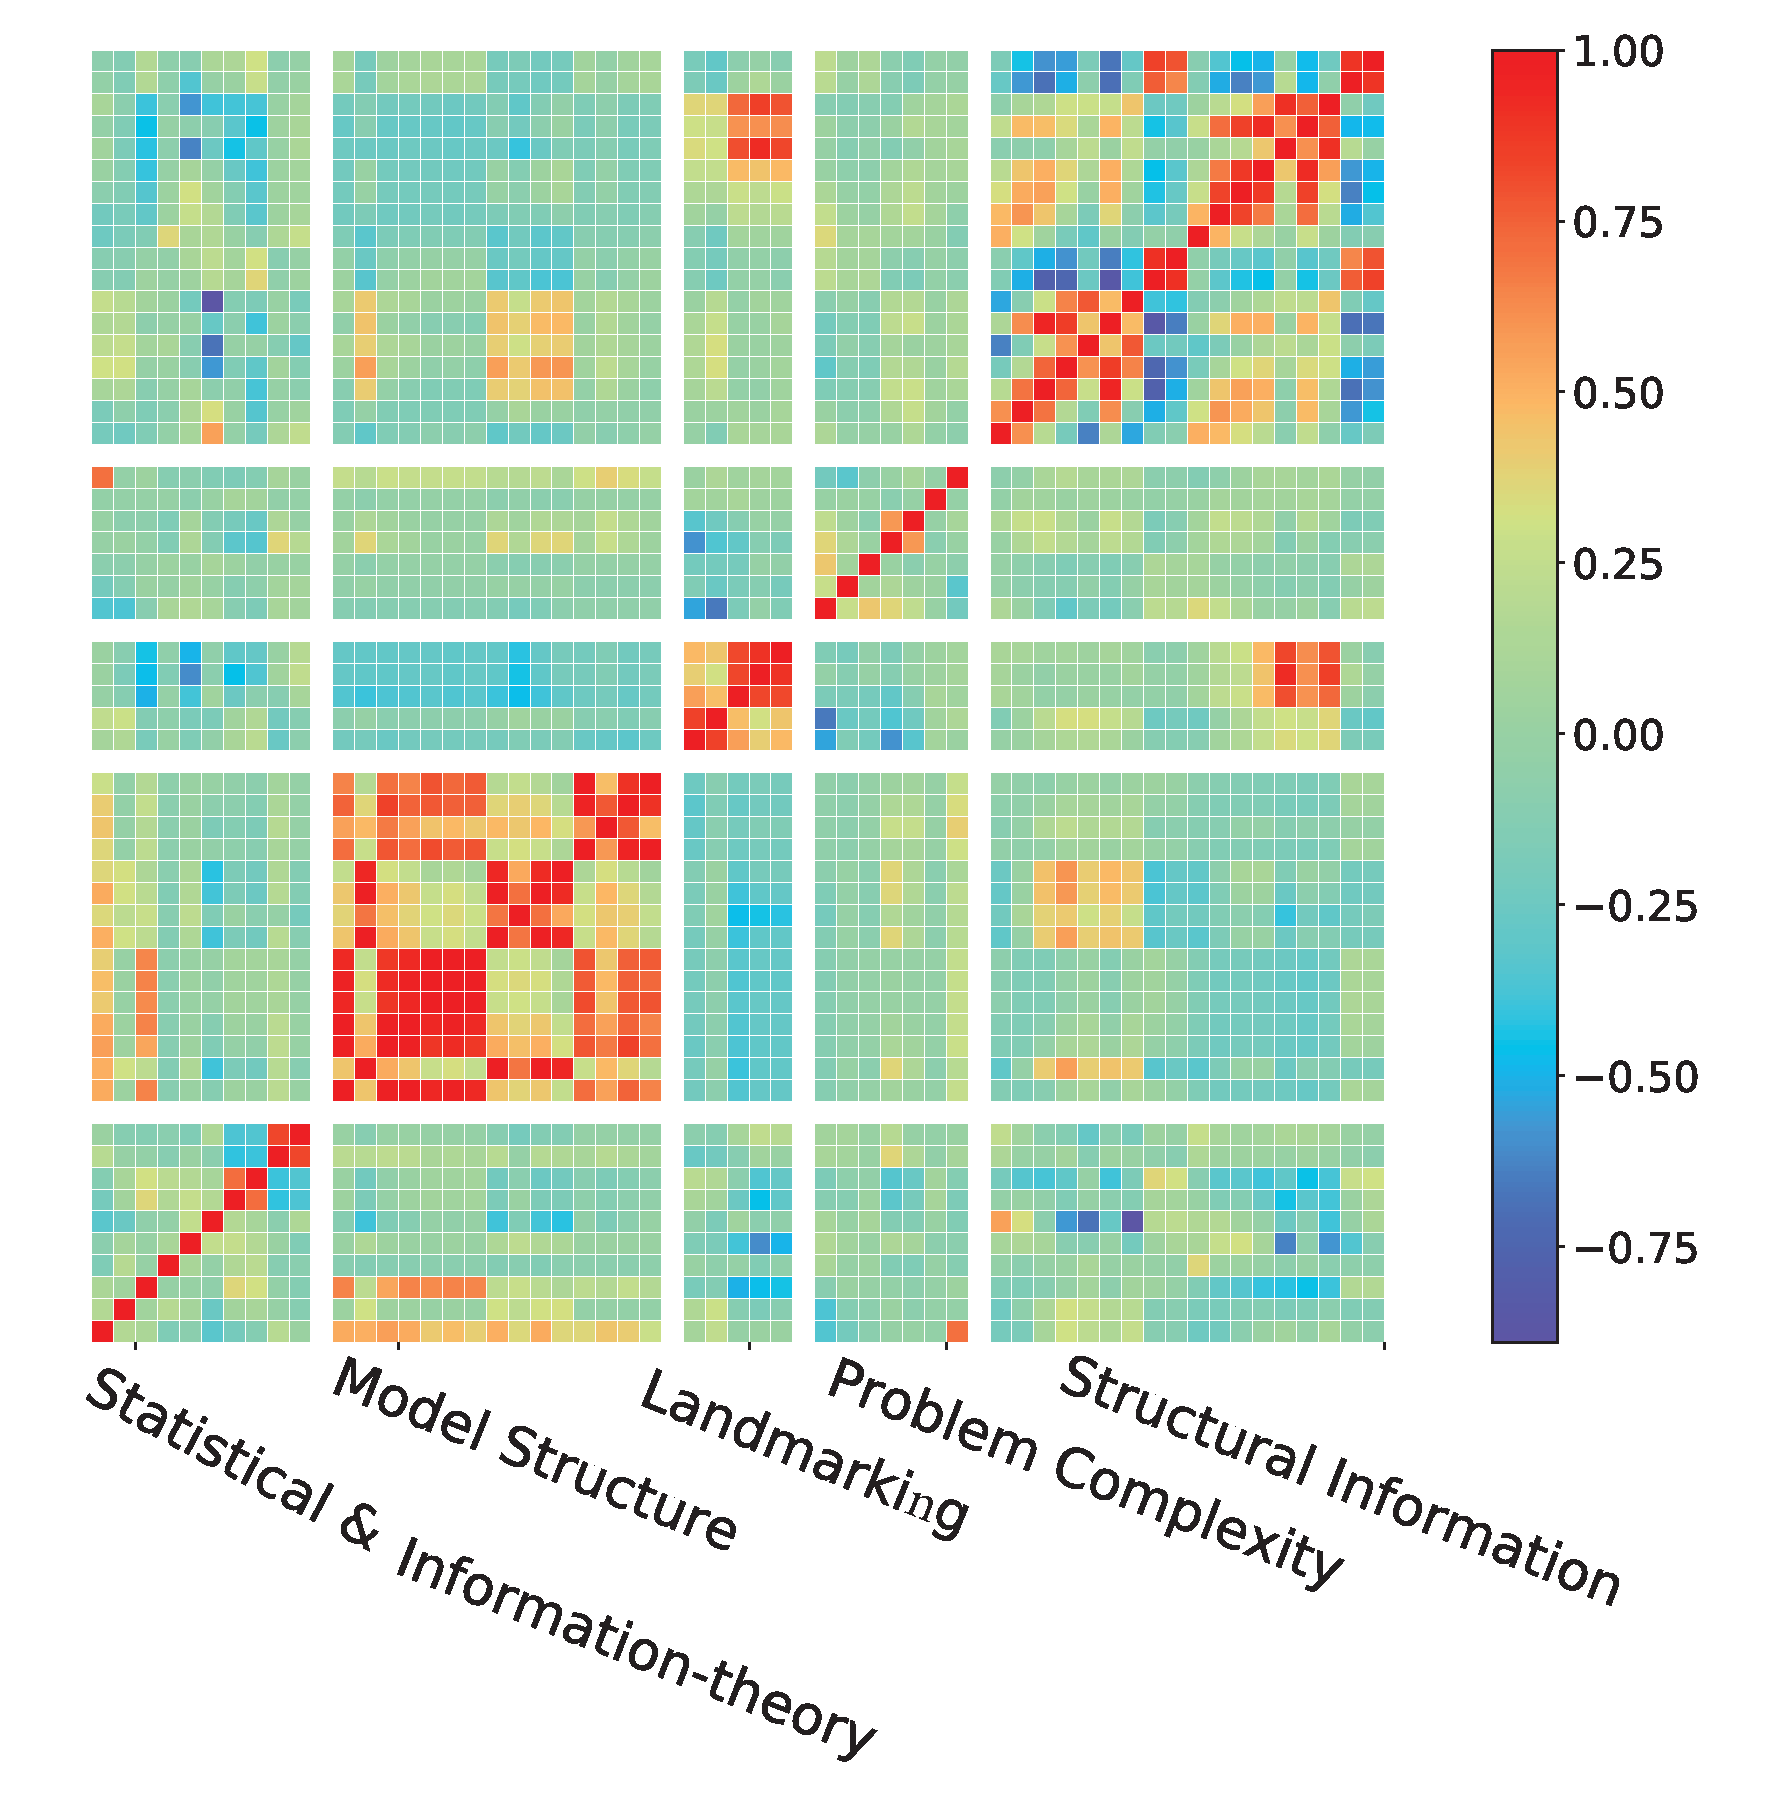
\includegraphics[width=7cm, height=6cm]{correlation.eps}
	\caption{Pearson's Linear Correlation Coefficients among Five Different Kinds of Meta features
		over 183 Classification Problems}
	\label{fig:correlation}
	%\normalsize
\end{figure}

1) Diverse base model construction
\label{Diverse}

There have been several different kinds of meta features in the field of algorithm recommendation \upcite{Wang2014A}. These meta features are extracted from different viewpoints of a classification problem independently. Figure \ref{fig:correlation} gives the correlation coefficients among the five kinds of meta feature groups extracted from 183 benchmark classification problems (see details in Appendix). These five kinds of meta feature groups include 1) statistical and information-theory based; 2) model structure based; 3) land marking based; 4) problem-complexity based; and 5) structural information based. 

From Figure \ref{fig:correlation}, we can find that the correlation among different kinds of meta features is quite low. This gives us an experimental evidence that different kinds of meta-features are independent with each other. Furthermore, it is more likely that different recommendation models constructed with these different kinds of meta features will be independent and diverse.

One way of the ensemble is to apply same models to different training data, while another is to apply different models on same training data. In this paper, the former is adopted. And to guarantee the diversity of Tier-1 learners, all combinations of different kinds of meta features are used to generate different Tier-1 training data, which also utilizes the complementary and diversity of meta features. And we use attribute selection method on Tier-2 training data to delete the redundant attributes (Tier-1 learners' output), which is equivalent to deleting corresponding Tier-1 learners, in order to promote base models' diversity further. 

2) Accurate base model construction
% 此论文是否已经确定使用mlknn作为基学习器,还是此论文提出了用于算法推荐的两层学习框架,基学习器任选(不重要)

There have been many different recommendation models constructed with respect to different kinds of meta features and single learning method\upcite{Ali2006On, Pise2016Algorithm, Yang2017Choosing, Lee2013Automatic, Ali2018A, Wang2014A, Zhu2018A}. To construct accurate base models, we can apply one of these recommendation models, which has not only good accuracy but also great generalization, as the base model of the ensemble on different training data. Furthermore, we deal with the recommendation problem as a multi-label problem, so \emph{ML-KNN} based recommendation model\upcite{Wang2014A} would be a good choice for that it's fast and accurate. 

As discussed in former item, the attribute selection method employed on Tier-2 training data will choose the attributes that are highly related with labels, which means that Tier-1 learners whose performance is better will be selected for recommendation. 

The above description provides us the evidence that it is feasible to construct a set of accurate base recommendation models of ensemble.



\subsection{Meta data extraction}
\label{meta data extraction}

Meta data extraction, as suggested by its name, is to extract meta data from the historical classification problems of $\mathcal{P}$ and the candidate classification algorithms set $\mathcal{A}$. It is composed of two procedures, meta target identification and meta feature collection. Each instance of meta data corresponds to a classification problem and consists of two parts: meta target and meta features.

For meta target identification, the appropriate algorithms refers to the best algorithm and the ones that have no significant difference with the best algorithm on a specific evaluation metric for the given $p_i \in \mathcal{P}$. Multiple comparison procedure \upcite{Toothaker1993Multiple,Demsar2006Statistical}, which has also been used in \cite{Wang2014A, Zhu2018A}, is utilized to identify meta target. The multiple comparison procedure is a statistical test method, which can identify a set of algorithms that are not significantly different from the best one in terms of a given metric (e.g., classification accuracy). These appropriate algorithms form the multi-label based meta target $Y_i = \{Y_{i,j} |1 \leq j \leq k \}$ of $p_i$ and $Y_{i,j}$ = 1 or 0 indicates the algorithm $a_j$ is appropriate or inappropriate for $p_i$.

For meta feature collection, all the $q$ different kinds of data characterization methods in $F$ are utilized on the historical classification problems to get $q$ groups of meta-features. It's a fact that different kinds of meta features reflect the properties of a classification problem in different viewpoint. Inspired by this idea, this paper attempts to construct the base recommendation learners with respect to different combinations of these meta features in a specific way, which also aims to utilize the complementarity of meta features effectively. 

\begin{algorithm}[!h]
%	\scriptsize
    \footnotesize
	\caption{Meta data extraction}
	\label{pro:Meta data}
	\begin{algorithmic}[1]
		
		\REQUIRE ~~\\
		$\mathcal{P}$: the historical classification problems, $\{p_i|i=1, 2, ..., n\}$ \\
		$\mathcal{A}$: the candidate classification algorithms, $\{a_j|j=1, 2, ..., k\}$ \\
		$F$: the set of meta feature extraction functions, $\{F_1, F_2, ..., F_q\}$\\ 
		%$nchoosek()$: the function to get all combinations\\
		\ENSURE ~~\\
		$\{D_1,D_2, ..., D_{2^q-1}\}$: the extracted meta datasets\\
		\STATE $D_1,D_2, ..., D_{2^q-1} = Null$;\\
		\FOR{each $p_i \in \mathcal{P}$ }
		\STATE $Y_i$ = targetIndentify($p_i$, $\mathcal{A}$);\\
		\FOR{each data characterization method $F_j \in F$}
		\STATE $X_i^j$ = featureCollect($p_i$, $F_j$);\\
		\STATE $X_i = X_i \cup X_i^j$;\\
		\ENDFOR
		\quad\scriptsize{//Therer are $q$ kinds of meta features}\\
		\STATE $X_i^{'} = \{X_{i,t} | 1 \leq t \leq 2^q - 1\} = nchoosek(\{X_i\})$;\\
		\quad\scriptsize{//There are $t = 2^q-1$ kinds of meta feature combinations}\\
		\FOR{each $X_{i,t} \in X_i^{'}$}
		\STATE $inst = (X_{i,t}, Y_i)$;\\
		\STATE $D_t = D_t \cup {inst}$;\\
		\ENDFOR
		\ENDFOR
		\STATE return $\{D_1,D_2, ..., D_{2^q-1}\}$;\\
	\end{algorithmic}
\end{algorithm}

Procedure \ref{pro:Meta data} gives pseudo code of meta data extraction. In this procedure, the three input parameters are the classification problems $\mathcal{P}$, candidate classification algorithms $\mathcal{A}$ and feature extraction functions $F$. The output of this procedure is multiple meta datasets, $\{D_1,D_2, ..., D_{2^q-1}\}$. In the procedure \ref{pro:Meta data}, first, meta datasets are initialized. For each historical classification problem $p_i \in \mathcal{P}$, its meta target $Y_i$ is identified and its meta features $X_i=\{X_i^j | 1 \leq j \leq q\}$ are collected in lines form 2 to 7. Each kind of meta features $X_i^j$ is extracted by corresponding method $F_j$. Secondly, all combinations of elements in $X_i$ are generated in line 8, that is, $X_i^{'} = \{X_{i,t} | 1 \leq t \leq 2^q - 1\} = nchoosek(\{X_i\})$. Here $nchoosek(Z)$ outputs all the possible combinations of the elements in $Z$. For example, let $Z=\{a, b, c\}$, then $nchoosek(Z)=\{\{a\}, \{b\}, \{c\}, \{a, b\}, \{a, c\}, \{b, c\}, \{a, b, c\}\}$. Next, for each $X_{i,t} \in X_i^{'}$, an instance $inst$, whose attribute is $X_{i,t}$ and label is $Y_i$, is generated and added to $D_t$. Finally, meta datasets $\{D_1,D_2, ..., D_{2^q-1}\}$ are returned. 

It is noted that, there are many methods to generate different combinations of meta features from the given $q$ kinds of meta features. The combination function $nchoosek()$ being chosen is due to the fact that it can not only generate multiple different sets of meta data for base learner construction, but also help to find whether the combinations of different kinds of meta features are better, and further discover the salient meta features for algorithm recommendation.

With the combination function $nchoosek()$ on $q$ different kinds of meta features, we can generate $\tau = 2^q - 1$ different meta feature combinations, which compose the features of $\tau$ different multi-label meta datasets. Finally, after meta data extraction, the historical classification problems $\mathcal{P}$ are transformed into meta datasets $\{D_1,D_2, ..., D_{2^q-1}\}$.


\subsection{Tier-1 and Tier-2 model construction}

This subsection depicts the process about Tier-1 and Tier-2 model construction based on meta datasets extracted in above section \ref{meta data extraction}. 

For convenience to describe, $L = \{L_t|1 \leq t \leq 2^q-1\}$ represents Tier-1 learners built on each meta dataset $D_t$. $Out = \{Out_t|1 \leq t \leq 2^q-1\}$ is the set of Tier-1 output datasets, where $Out_t$ is produced by $L_t$. $D^2 =\{D^2_j|1 \leq j \leq k\}$ represents the set of Tier-2 training datasets which are transformed from Tier-1 output. And $D^2_j$ will be used to construct a Tier-2 model $M^2_j$ to judge whether algorithm $a_j$ is appropriate for the new classification problem. 


\begin{algorithm}[!h]
	%\scriptsize
	\footnotesize
	\caption{Tier-1 and Tier-2 model construction}
	\label{pro:model construction}
	\begin{algorithmic}[1]
		
		\REQUIRE ~~\\
		${D}$: the set fo meta datasets, $D =\{D_t|1 \leq t \leq 2^q-1\}$ \\
		$MLkNN$: the multi-label classification algorithm \emph{ML-KNN} \\
		$L$: the set of untrained Tier-1 learners, $L = \{L_t|1 \leq t \leq 2^q-1\}$\\
		\ENSURE ~~\\
		$L^{'}$: the set of selected trained Tier-1 learners, $L^{'} = \{L_t^{'}|1 \leq t \leq m\}$\\
		$M^2$: the Tier-2 classification model, $M^2 =\{M^2_j|1 \leq j \leq k\}$\\
		\STATE $Out = \{Out_1,Out_2, ...,Out_{2^q-1}\} = Null$;
		\STATE $D^2 = \{D^2_1,D^2_2, ..., D^2_k\} = Null$;
		\FOR{each $L_t \in L$}
		\STATE $L_t = MLkNN.build(D_t)$;\quad\scriptsize{//Tier-1 learner construction}\\
		\ENDFOR
		\FOR{each $D_t \in D$}
		\FOR{each $inst_i \in D_t$}
		\STATE $\{v(i,1),v(i,2), ...,v(i,k)\} = L_t.predict(inst_i)$;\\
		\STATE $Out_t = Out_t \cup {\{v(i,1),v(i,2), ...,v(i,k)\}}$;\\
		\ENDFOR
		\ENDFOR
		\STATE $D^2 = transform(Out)$;\\
		\FOR{each instance $D^2_j\in D^2$}
		\FOR{each instance $inst_i\in D^2_j$}
		\STATE $inst_i.label(i,j) = Y_{i,j}$;\\
		\ENDFOR
		\ENDFOR
		\FOR{each $D^2_j \in D^2$}
		\STATE $D^{2'}_j = featureSelect(D^2_j)$;\\
		\FOR{each $attribute_t \in D^2_j$}
		\IF{$attribute_t$ is selected}
		\STATE $L^{'} = L^{'} \cup L_t$
		\ENDIF
		\ENDFOR
		\STATE $M^2_j.build(D^{2'}_j)$;\quad\scriptsize{//Tier-2 model construction}\\
		\ENDFOR
		\STATE return $L^{'}$ and $M^2$;\\
	\end{algorithmic}
\end{algorithm}  


The pseudo code of Tier-1 and Tier-2 model construction is given in the procedure \ref{pro:model construction}. First, the Tier-1 base learners are built over the meta datasets $\{D_t|1 \leq t \leq 2^q-1\}$ in lines from 3 to 5, where meta instances corresponding to the same historical classification problem $p_i$ have different attributes(meta features) but same labels(meta target). As can be seen in framework \ref{fig:Framework}, Tier-1 learner construction is identical and simply. Each $L_t$ is trained based on each corresponding meta dataset $D_t$ by \emph{ML-KNN}. After model constructing, each instance is predicted by each corresponding Tier-1 learner in lines from 6 to 11, that is, each instance of $D_t$ is not only used to build base model $L_t$, but also predicted by $L_t$ to generate $Out_t$. Then the prediction output datasets $\{Out_1,Out_2, ...,Out_{2^q-1}\}$ of Tier-1 model are transformed to Tier-2 training datasets $\{D^2_1, D^2_2, ..., D^2_k\}$ in lines from 13 to 15 as shown in Figure \ref{tier-2_data_generation}. Each instance of $D^2_j$ is labeled in lines from 16 to 18. After Tier-2 training data generated, each Tier-2 dataset $D^2_j$ is first selected useful features in line 19 and then applied to construct a Tier-2 model $M^2_j$ in line 20. Finally, Tier-1 selected trained learners $L^{'} = \{L_t^{'}|1 \leq t \leq m\}$ and Tier-2 binary classification model $M^2 =\{M^2_j|1 \leq j \leq k\}$ is returned to recommend algorithm(s) for a new classification problem.

It's noted that, before constructing a binary classification model, we conduct attribute selection to $D^2_j$ for the following three reasons:

\begin{itemize}
	\item It will remove redundant and irrelevant attributes that may lead to the loss of the binary classification performance. Because each attribute is produced by each Tier-1 learner, removing redundant and irrelevant attributes is equivalent to selecting diverse and accurate Tier-1 learners to achieve better ensemble learning. 
	
	\item It will help us to find which combination of meta feature is more useful, since different meta datasets only have different attributes but have same labels.
	
	\item With less attributes, less Tier-1 learners will be utilized to generate the Tier-2 attributes for a new classification problem and thus reduce the consuming time in the recommendation procedure.
\end{itemize}

In the \emph{EML} algorithm, CFS\upcite{Hall1999Correlation} attribute selection method with the BestFirst\upcite{korf1993linear} search strategy are employed.

\begin{figure}[!h]
	\small
	\centering
	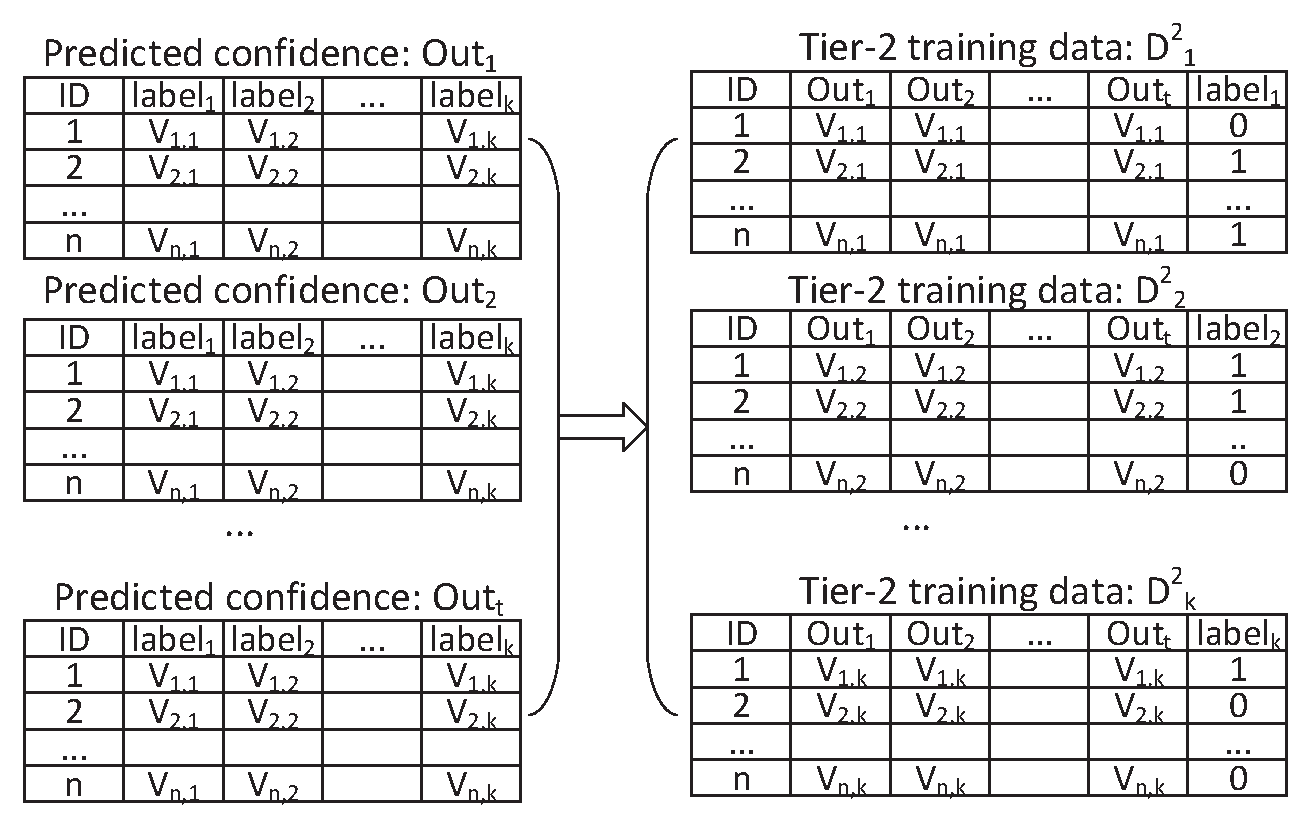
\includegraphics[width=7cm, height=5.5cm]{tier-2_data_generation.eps}
	\caption{Tier-2 training data generation based on Tier-1 models' output}
	\label{tier-2_data_generation}
	%\normalsize
\end{figure}

Figure \ref{tier-2_data_generation} displays the transformation from Tier-1 output $Out$ to Tier-2 input $D^2$. In this figure, ID number represents each meta instance corresponding to each classification problem $p_i$ and $label_k$ is the $k_{th}$ label of meta data corresponding to each classification algorithm $a_k$. $v_{i,k}$ is the confidence of $label_k$ in the $i_{th}$ instance, which is predicted by corresponding Tier-1 learner. 

Each table in the left part of Figure \ref{tier-2_data_generation} represents the output $Out_t$ of each Tier-1 learner $L_t$, and each table in the right part represents the Tier-2 training dataset $D^2_j$ for each label $label_j$. $v_(i,j) \in Out_t$ is the confidence of $label_j$ of the $i_{th}$ instance predicted by $L_t$, which will be transformed as $v_(i,t) \in D^2_j$. In other words, all the $j_{th}$ column of $Out_t \in Out$ are incorporated together as attributes of $D^2_j$. In addition, $label_{i,j}$ of $D^2_j$ is meta target $Y_{i,j} \in Y_i$ and $label_{i,j}$ = 1 or 0 indicates the algorithm $a_j$ is appropriate or inappropriate on $p_i$. 

The reason why we generate Tier-2 training dataset $D^2_j$ for each algorithm $a_j$ respectively, instead of combining them into a whole, is shown in Figure \ref{Confidence comparison}.

\begin{figure}[!h]
	\small
	\centering
	\scalebox{1.0}{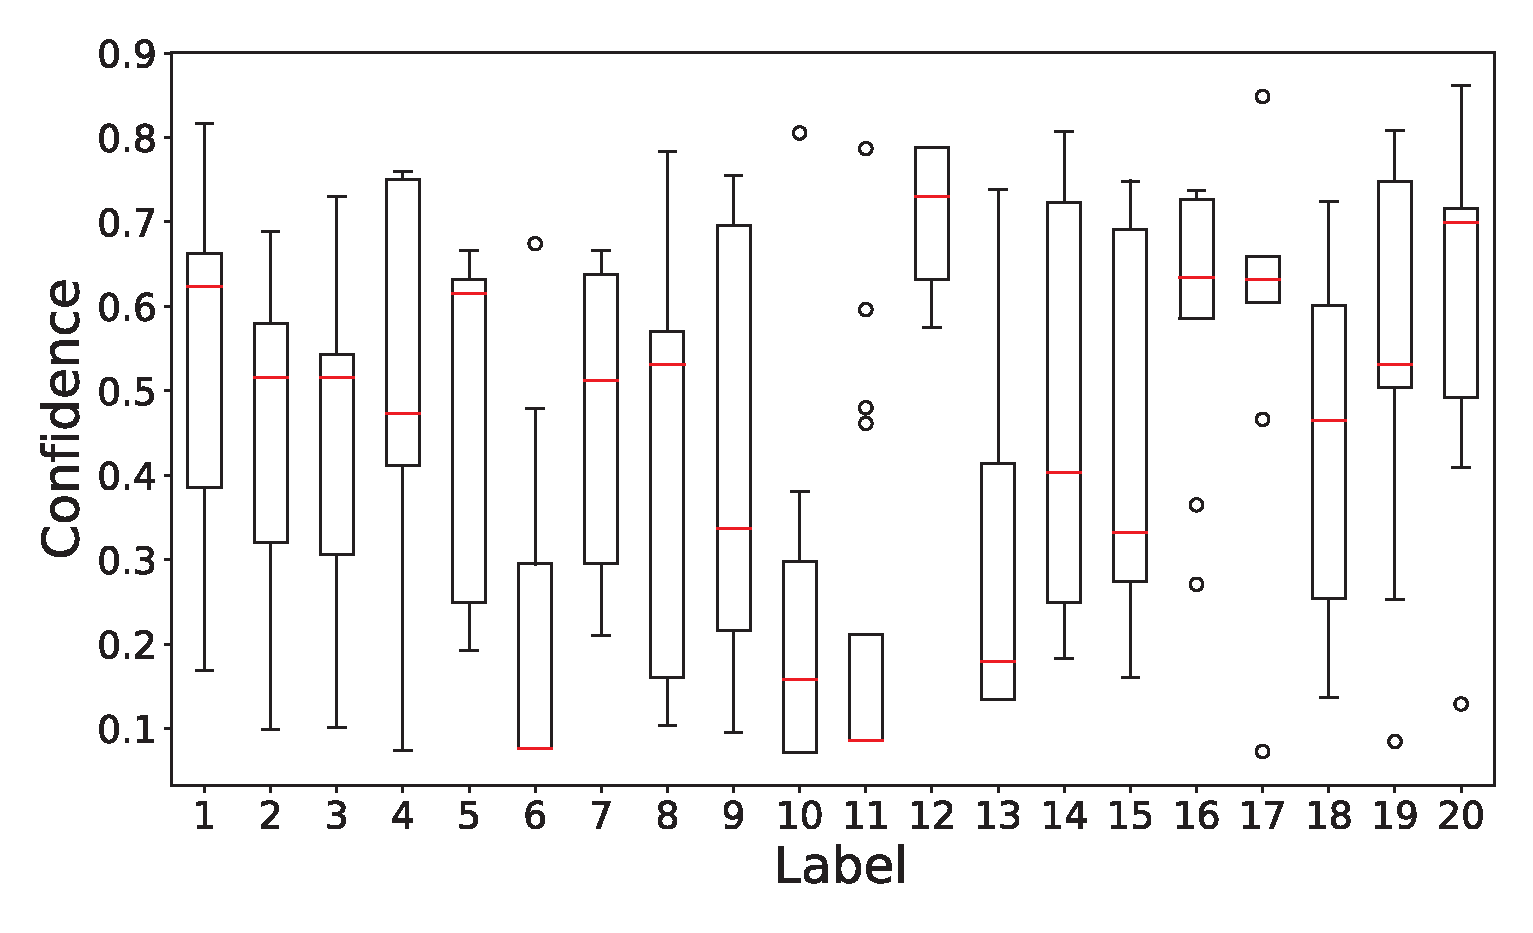
\includegraphics[width=7cm, height=3.5cm]{28.eps}}
	\caption{Confidence comparison between different labels}
	\label{Confidence comparison}
	%\normalsize
\end{figure} 

Figure \ref{Confidence comparison} compares the predicted confidence values between different labels on the same meta data, whose attributes are the combination of all five kinds of meta features and target is identified in terms of classification accuracy. 20 classification algorithms are employed, so the number of label is 20 in X-axis and Y-axis depicts the confidence value range. 

In this figure, each separate box is produced by the “boxplot” for each label according to its confidence values produced on the meta data by same \emph{ML-KNN}. And the circles are outliers. We can observe that the confidence values of different labels have obviously different distributions, like $label_5$, $label_{11}$, $label_{12}$, etc.. Whereby, it would be better to learn respectively to predict each label as discussed above. Furthermore, C4.5\upcite{Quinlan1993Programs} + AdaBoost\upcite{Freund1995A} is adopted to build each binary classification model \emph{$M^2_j \in M^2$} in \emph{EML}. 


\subsection{Recommendation based on ensemble learning}

This subsection describes how to recommend appropriate algorithm(s) for a new classification problem.

As described above, Tier-1 selected trained learners $L^{'}$ and Tier-2 binary classification models $M^2 =\{M^2_j|1 \leq j \leq k\}$ are constructed based on meta data, which form an ensemble learner to recommend algorithms.

The pseudo code of recommendation based on ensemble learning is shown in Procedure \ref{algo:recommendation}. There are 5 input parameters in this procedure. $p_{new}$ is the new classification problem, $\mathcal{A}$ is the set of candidate classification algorithms, $F$ is the set of meta feature extraction functions, $L^{'}$ is the set of selected trained Tier-1 learners and $M^2$: the Tier-2 binary classification model. The output of the procedure \emph{$Algs$} is the set of recommended appropriate algorithms for $p_{new}$.

\begin{algorithm}[!h]
	%\scriptsize
	\footnotesize
	\caption{Recommendation based on ensemble learning}\label{algo:recommendation}
	
	\begin{algorithmic}[1]
		\REQUIRE ~~\\
		$p_{new}$: the new classification problem \\
		$\mathcal{A}$: the candidate classification algorithms, $\{a_j|j=1, 2, ..., k\}$ \\
		$F$: the set of meta feature extraction functions, $\{F_1, F_2, ..., F_q\}$\\ 
		%$nchoosek()$: the function to get all combinations\\
		%$featureSelect$: the method to select useful attributes of $D^2$\\
		$L^{'}$: the set of selected trained Tier-1 learners\\
		$M^2$: the Tier-2 classification model, $M^2 =\{M^2_j|1 \leq j \leq k\}$\\
		\ENSURE ~~\\
		$Algs$: set of recommended appropriate algorithms for $p_{new}$\\
		\FOR{each data characterization method $F_j$ in $F$}
		\STATE $X_{new}^j$ = featureCollect($p_{new}$, $F_j$);\\
		\STATE $X_{new} = X_{new} \cup X_{new}^j$;\\
		\ENDFOR
		\STATE $X_{new}^{'} = \{X_{new,t} | 1 \leq t \leq 2^q - 1\} = nchoosek(\{X_{new}\})$;\\
		\FOR{each $X_{new,t} \in X_{new}^{'}$}
		\STATE $inst_t = (X_{new,t}, '?')$;\\
		\STATE $D_{new} = D_{new} \cup {inst_t}$;\\
		\ENDFOR
		\STATE $Out_{new} = L^{'}.predict(D_{new})$;\\
		\STATE $D^2_{new} = transform(Out_{new})$;\\	
		\FOR{ each instance $inst_j \in D^{2'}_{new}$}
		\STATE $C_j = classify(M^2_j, inst_j)$;\\
		\IF{$C_j$ == 1}
		\STATE $Algs = Algs \cup \{a_j\}$;\\
		\ENDIF
		\ENDFOR
		\STATE return $Algs$;\\
	\end{algorithmic}
\end{algorithm}

 In Procedure \ref{algo:recommendation}, a new classification problem $p_{new}$ first is collected $q$ kinds of meta features to form its feature set $X_{new}$ in lines from 1 to 4. Then all combinations of elements in $X_{new}$ are given by function $nchoosek$ in line 5, which underlie $D_{new}$ as its attributes in lines from 6 to 9. The unknown labels of $D_{new}$ are set as '?'. Next, Tier-1 model output $Out_{new}$ is generated by $L^{'}$ on $D_{new}$ in  line 10 and then transformed to Tier-1 model input $D^2_{new}$ in line 11. In lines from 12 to 17, $M^2_j$ classifies each instance $inst_j$ in $D^2_{new}$ to obtain label $C_j$. If $C_j$ == 1, the corresponding algorithm $a_j$ will be added to $Algs$. Finally, the set of recommended appropriate algorithms $Algs$ for $p_{new}$ is returned, which indicates that the recommendation process is over.

\section{Empirical Study}
\label{experiment}

To evaluate the effectiveness of the \emph{EML} method, an empirical study is conducted in this section. Firstly, the experimental setup is explained. Then, performance of \emph{EML} is compared with the base line methods. And finally, the comparison on th number of recommended algorithms among \emph{EML} and baseline methods is presented.%Next, usage of the combinations of meta features are summarized. Then performance of $E-MLKNN_{ns}$ (\emph{EML} without classifying each label separately) is compared with \emph{EML}. And finally, parameter sensitivity is analyzed.

\subsection{Experimental setup}

To guarantee the reproducibility of the experiment, we set up our experiment as follows.

\subsubsection{Benchmark datasets}

In the experiment, 183 publicly available datasets are used, which are  from UCI repository\upcite{Dua2019UCI}, StatLib\upcite{Pantelis2005}, openML\upcite{OpenMLR2017}, KEEL\upcite{alcala2011keel}. Table in appendix gives the statistical summary of the datasets, including their names, number of features, instances and classes. These datasets are widely used in classification field and representative for the classification problem in practical. 		


%		\begin{table*}[]
%			\centering
%			\scalebox{1.15}{
%			\begin{threeparttable}
%				\tiny			
%				\caption{Description of the Benchmark datasets}
%				\label{table:dataset}
%				\begin{tabular}{p{0.1cm}lp{0.6cm}<{\centering}p{0.6cm}<{\centering}p{0.6cm}<{\centering}|p{0.1cm}lp{0.6cm}<{\centering}p{0.6cm}<{\centering}p{0.6cm}<{\centering}}
%					\hline																			
%					ID	&	Name	&	\#Features	&	\#Instances	&	\#Classes	&	ID	&	Name	&	\#Features	&	\#Instances	&	\#Classes	\\ \hline
%					1	&	abalone	&	8	&	4177	&	29	&	93	&	landsat\_train	&	36	&	4435	&	6	\\
%					2	&	adellll	&	21	&	1075	&	4	&	94	&	led7digit	&	7	&	500	&	10	\\
%					3	&	advertisement	&	1558	&	3279	&	2	&	95	&	letter	&	16	&	20000	&	26	\\
%					4	&	analcatdata\_assessment	&	15	&	13	&	4	&	96	&	liver\_disorders	&	6	&	345	&	2	\\
%					5	&	analcatdata\_authorship	&	70	&	841	&	4	&	97	&	lung\_cancer	&	56	&	32	&	3	\\
%					6	&	analcatdata\_bankruptcy	&	6	&	50	&	2	&	98	&	lymph	&	18	&	148	&	4	\\
%					7	&	analcatdata\_birthday	&	3	&	365	&	7	&	99	&	magic04	&	10	&	19020	&	2	\\
%					8	&	analcatdata\_bondrate	&	11	&	57	&	5	&	100	&	mammographic\_masses	&	5	&	961	&	2	\\
%					9	&	analcatdata\_boxing1	&	3	&	120	&	2	&	101	&	marketing	&	13	&	6876	&	9	\\
%					10	&	analcatdata\_boxing2	&	3	&	132	&	2	&	102	&	messidor\_features	&	19	&	1151	&	2	\\
%					11	&	analcatdata\_braziltourism	&	8	&	412	&	7	&	103	&	mfeat\_factors	&	216	&	2000	&	10	\\
%					12	&	analcatdata\_broadway	&	9	&	95	&	5	&	104	&	mfeat\_fourier	&	76	&	2000	&	10	\\
%					13	&	analcatdata\_broadwaymult	&	7	&	285	&	7	&	105	&	mfeat\_karhunen	&	64	&	2000	&	10	\\
%					14	&	analcatdata\_chall101	&	2	&	138	&	2	&	106	&	mfeat\_morphological	&	6	&	2000	&	10	\\
%					15	&	analcatdata\_creditscore	&	6	&	100	&	2	&	107	&	mfeat\_pixel	&	240	&	2000	&	10	\\
%					16	&	analcatdata\_currency	&	3	&	31	&	7	&	108	&	mfeat\_zernike	&	47	&	2000	&	10	\\
%					17	&	analcatdata\_cyyoung8092	&	10	&	97	&	2	&	109	&	molecular\_biology\_promoters	&	58	&	106	&	2	\\
%					18	&	analcatdata\_cyyoung9302	&	10	&	92	&	2	&	110	&	monks\_problems\_1\_test	&	6	&	122	&	2	\\
%					19	&	analcatdata\_dmft	&	4	&	797	&	6	&	111	&	monks\_problems\_1\_train	&	6	&	124	&	2	\\
%					20	&	analcatdata\_draft	&	5	&	365	&	12	&	112	&	monks\_problems\_2\_test	&	6	&	432	&	2	\\
%					21	&	analcatdata\_esr	&	2	&	32	&	2	&	113	&	monks\_problems\_2\_train	&	6	&	169	&	2	\\
%					22	&	analcatdata\_halloffame	&	17	&	1340	&	3	&	114	&	monks\_problems\_3\_test	&	6	&	432	&	2	\\
%					23	&	analcatdata\_homerun	&	27	&	162	&	2	&	115	&	monks\_problems\_3\_train	&	6	&	122	&	2	\\
%					24	&	analcatdata\_lawsuit	&	4	&	264	&	2	&	116	&	movement\_libras	&	90	&	360	&	15	\\
%					25	&	analcatdata\_mapleleafs	&	1	&	84	&	3	&	117	&	mushroom	&	22	&	8124	&	2	\\
%					26	&	analcatdata\_marketing	&	32	&	343	&	5	&	118	&	newthyroid	&	5	&	215	&	3	\\
%					27	&	analcatdata\_reviewer	&	8	&	329	&	3	&	119	&	nomao	&	118	&	10339	&	2	\\
%					28	&	analcatdata\_votesurvey	&	4	&	48	&	4	&	120	&	nursery	&	8	&	12960	&	5	\\
%					29	&	anneal.ORIG	&	38	&	898	&	6	&	121	&	onehr	&	72	&	2536	&	2	\\
%					30	&	anneal	&	38	&	798	&	5	&	122	&	optdigits	&	64	&	3823	&	10	\\
%					31	&	arrhythmia	&	279	&	452	&	16	&	123	&	page\_blocks	&	10	&	5473	&	5	\\
%					32	&	audiology	&	69	&	226	&	24	&	124	&	parkinson Speech	&	26	&	1040	&	2	\\
%					33	&	australian	&	14	&	690	&	2	&	125	&	pendigits	&	16	&	10992	&	10	\\
%					34	&	autism\_Adolescent\_Data	&	20	&	104	&	2	&	126	&	phishing	&	30	&	11055	&	2	\\
%					35	&	autism\_Adult\_Data	&	20	&	704	&	2	&	127	&	phoneme	&	5	&	5404	&	2	\\
%					36	&	autism\_Child\_Data	&	20	&	292	&	2	&	128	&	PimaIndDia	&	8	&	768	&	2	\\
%					37	&	autos	&	25	&	205	&	7	&	129	&	post\_oper	&	8	&	90	&	3	\\
%					38	&	bach\_chorals\_harmony	&	16	&	5665	&	102	&	130	&	primary\_tumor	&	17	&	339	&	22	\\
%					39	&	backache	&	32	&	180	&	2	&	131	&	qualBank	&	6	&	250	&	2	\\
%					40	&	balance\_scale	&	4	&	625	&	3	&	132	&	ring	&	20	&	7400	&	2	\\
%					41	&	banana	&	2	&	5300	&	2	&	133	&	saheart	&	9	&	462	&	2	\\
%					42	&	bands	&	19	&	365	&	2	&	134	&	satimage	&	36	&	6435	&	7	\\
%					43	&	bank\_full	&	16	&	13563	&	2	&	135	&	seeds	&	7	&	210	&	3	\\
%					44	&	blood\_transfusion	&	4	&	748	&	2	&	136	&	segment	&	19	&	2310	&	7	\\
%					45	&	breast\_cancer	&	9	&	286	&	2	&	137	&	seismic\_bumps	&	18	&	2584	&	2	\\
%					46	&	breast\_w	&	9	&	699	&	2	&	138	&	semeion	&	256	&	1593	&	10	\\
%					47	&	bridges\_version1	&	11	&	105	&	6	&	139	&	shuttle	&	9	&	13050	&	7	\\
%					48	&	bridges\_version2	&	11	&	105	&	6	&	140	&	sick	&	29	&	3772	&	2	\\
%					49	&	bupa	&	6	&	345	&	2	&	141	&	skin	&	3	&	19604	&	2	\\
%					50	&	car	&	6	&	1728	&	4	&	142	&	solar\_flare\_1	&	12	&	323	&	6	\\
%					51	&	census\_income	&	14	&	16280	&	2	&	143	&	solar\_flare\_2	&	12	&	1066	&	6	\\
%					52	&	chess	&	6	&	11222	&	18	&	144	&	sonar	&	60	&	208	&	2	\\
%					53	&	chronic\_kidney\_disease\_full	&	24	&	400	&	2	&	145	&	soybean	&	35	&	683	&	19	\\
%					54	&	clean1	&	168	&	476	&	2	&	146	&	spambase	&	57	&	4601	&	2	\\
%					55	&	cmc	&	9	&	1473	&	3	&	147	&	spectf\_test	&	44	&	269	&	2	\\
%					56	&	colic	&	22	&	368	&	2	&	148	&	spectf\_train	&	44	&	80	&	2	\\
%					57	&	colic\_ORIG	&	27	&	368	&	2	&	149	&	spect\_test	&	22	&	187	&	2	\\
%					58	&	connect\_4	&	42	&	13511	&	3	&	150	&	spect\_train	&	22	&	80	&	2	\\
%					59	&	contraceptive	&	9	&	1473	&	3	&	151	&	splice	&	61	&	3190	&	3	\\
%					60	&	credit\_a	&	15	&	690	&	2	&	152	&	sponge	&	45	&	76	&	3	\\
%					61	&	credit\_g	&	24	&	1000	&	2	&	153	&	student\_mat	&	30	&	395	&	21	\\
%					62	&	crx	&	15	&	653	&	2	&	154	&	student\_por	&	30	&	649	&	21	\\
%					63	&	cylinder\_bands	&	39	&	540	&	2	&	155	&	synthetic\_control	&	60	&	600	&	6	\\
%					64	&	dermatology	&	34	&	366	&	6	&	156	&	tae	&	5	&	151	&	3	\\
%					65	&	diabetes	&	8	&	768	&	2	&	157	&	texture	&	40	&	5500	&	11	\\
%					66	&	dr	&	19	&	1151	&	2	&	158	&	thoraricSurgery	&	16	&	470	&	2	\\
%					67	&	echocardiogram	&	11	&	75	&	3	&	159	&	thyroid	&	21	&	7200	&	3	\\
%					68	&	ecoli	&	7	&	336	&	8	&	160	&	tic\_tac\_toe	&	9	&	958	&	2	\\
%					69	&	eegEyeState	&	14	&	14980	&	2	&	161	&	titanic	&	3	&	2201	&	2	\\
%					70	&	flag	&	28	&	194	&	8	&	162	&	trains	&	32	&	10	&	2	\\
%					71	&	flare	&	11	&	1066	&	6	&	163	&	twonorm	&	20	&	7400	&	2	\\
%					72	&	forestType	&	27	&	198	&	4	&	164	&	urbanland\_test	&	147	&	507	&	9	\\
%					73	&	german	&	20	&	1000	&	2	&	165	&	urbanland\_train	&	147	&	168	&	9	\\
%					74	&	glass	&	9	&	214	&	7	&	166	&	vehicle	&	18	&	846	&	4	\\
%					75	&	haberman	&	3	&	306	&	2	&	167	&	vertebral\_2c	&	6	&	310	&	2	\\
%					76	&	hayes\_roth\_test	&	4	&	28	&	4	&	168	&	vertebral	&	6	&	310	&	3	\\
%					77	&	hayes\_roth\_train	&	4	&	132	&	4	&	169	&	vote	&	16	&	435	&	2	\\
%					78	&	heart\_c	&	13	&	303	&	5	&	170	&	vowel	&	13	&	990	&	11	\\
%					79	&	heart\_h	&	13	&	294	&	5	&	171	&	wall\_follow24	&	24	&	5456	&	4	\\
%					80	&	heart\_statlog	&	13	&	270	&	2	&	172	&	wall\_follow4	&	4	&	5456	&	4	\\
%					81	&	hepatitis	&	19	&	155	&	2	&	173	&	waveform\_5000	&	40	&	5000	&	3	\\
%					82	&	housevotes	&	16	&	232	&	2	&	174	&	wdbc	&	30	&	569	&	2	\\
%					83	&	hypothyroid	&	29	&	3772	&	4	&	175	&	wholesale	&	7	&	440	&	2	\\
%					84	&	ilpd	&	10	&	583	&	2	&	176	&	wilt\_test	&	5	&	500	&	2	\\
%					85	&	ionosphere	&	34	&	351	&	2	&	177	&	wilt\_train	&	5	&	4339	&	2	\\
%					86	&	iris	&	4	&	150	&	3	&	178	&	wine	&	13	&	178	&	3	\\
%					87	&	kdd\_JapaneseVowels\_test	&	14	&	5687	&	9	&	179	&	winequality\_red	&	11	&	1599	&	10	\\
%					88	&	kdd\_JapaneseVowels\_train	&	14	&	4274	&	9	&	180	&	winequality\_white	&	11	&	4898	&	10	\\
%					89	&	kdd\_synthetic\_control	&	61	&	600	&	6	&	181	&	wisconsin	&	9	&	683	&	2	\\
%					90	&	kr\_vs\_kp	&	36	&	3196	&	2	&	182	&	yeast	&	8	&	1484	&	13	\\
%					91	&	labor	&	16	&	57	&	2	&	183	&	zoo	&	16	&	101	&	7	\\
%					92	&	landsat\_test	&	36	&	2000	&	6	&		&		&		&		&		\\ \hline
%					
%				\end{tabular}
%			\end{threeparttable}}
%		\end{table*}


\subsubsection{Candidate classification algorithms}

To make the experimental results in this paper more generalized, we employ 20 well known classification algorithms and they are put forward based on different mechanisms. The algorithms are categorized as follows.

\begin{itemize}
	\item Probability-based algorithms: Aggregating One-Dependence Estimators (AODE), Naive Bayes (NB), Bayes Network;
	\item Tree-based algorithms: C4.5, CART, Random Tree;
	\item Rule-based algorithms: Ripper, PART, OneR, NNge;
	% \item Neural network-based algorithm: MLP;
	\item Support-vector-machine-based algorithm: SMO;
	\item Lazy learning-based algorithm: IB1;
	\item Gaussian function-based algorithm: RBF-Network;
	\item Ensemble learning-based algorithms: RandomForest, Boosting+NB, Boosting+C4.5, Boosting+PART, Bagging+NB, Bagging+C4.5, Bagging+PART.
\end{itemize}

\subsubsection{Metrics to evaluate the performance of the candidate classification algorithms}

In our experiment, two kinds of metrics are used to evaluate the performance of the candidate classification algorithms. One is the commonly used metric $ accuracy $ and the other is $ ARR\ (Adjusted\ Ratio\ of\ Ratios) $\upcite{Brazdil2003Ranking} which considers both the classification accuracy and runtime. %$ ARR $ can be computed by formulas \ref{arr1} and \ref{arr2}:

%\begin{figure*}
%\begin{equation}
%ARR _{A_{i},A_{j}}^{D_{k}} = \dfrac{acc_{i}^{k}/acc_{j}^{k}}{1+\alpha\cdot log(t_{i}^{k}/t_{j}^{k})}(1\leq i\neq j\leq m,1\leq k \leq n)
%\label{arr1}
%\end{equation}
%\begin{equation}
%ARR_{A_{i}}^{D_{k}}=\dfrac{1}{m-1}\varSigma_{j=1\wedge j\neq i}^{m}ARR_{A_{i},A_{j}}^{D}(1\leq i\neq j\leq m,1\leq k \leq n)
%\label{arr2}
%\end{equation}
%\end{figure*}

%In Formulas \ref{arr1} and \ref{arr2}, $ m $ is the number of candidate classification algorithms while $ n $ is the number of datasets. $ acc_{i}^{k} $ and $ t_{i}^{k} $ denote the classification accuracy and runtime of algorithm $ A_{i} $ on dataset $ d_{k} $ respectively. $ \alpha $ is the trade-off coefficient between the classification accuracy and runtime, which is set to 0.05\% and 0.1\% in this paper.

What's more, a 5$ \times $10-folds cross-validation procedure is performed when evaluating the classification algorithms on the given dataset.% On one hand, this procedure can control the variation due to the different choices of training and testing datasets, and on the other hand, the performance metrics estimated by this procedure can be further used in multiple comparison procedure for recognizing the appropriate algorithms of a given dataset.

%\subsubsection{Link prediction methods}
%
%To describe the relation of the dataset and algorithm node pair from different perspectives, we employ 22 link prediction methods based on varieties of mechanisms, which are:
%		
%  \begin{itemize}
%		\item Local information based: CN, Salton Index, Jaccard, Sorensen, HPI, HDI, LHN, AA, RA, PA.
%		
%		\item Local Naive bayes based: LNBCN, LNBAA, LNBRA.
%		
%		\item Path based: LocalPath, Katz, LHN2
%		
%		%\item Random walk based: ACT (Average Commute Time)\upcite{Klein1993Resistance}, 
%		\item Random walk based: RWR, LRW, SRW.
%		
%		\item Others: MFI, TSCN, TSAA (AA based transferring similarity).
%  \end{itemize}

\subsubsection{Baseline methods and performance measures}

%% this will be changed when the experiment is ending
The proposed \emph{EML} method is compared to another two multi-label based classification algorithm recommendation method, the \emph{ML-KNN} based method\upcite{Wang2014A} and the single link prediction based method \emph{SLP}\upcite{Zhu2018A}, which only utilize a single link prediction algorithm in recommendation. In this experiment, $ RWR $\upcite{liu2010link} is used as the link prediction methods in \emph{SLP} and its names is used to represent the corresponding \emph{SLP} based recommendation methods. %including $ Katz $, $ LRW $ and $ SRW $, which represent three variants of the single link prediction based method that utilize the corresponding link prediction methods in recommendation\upcite{Zhu2018A} and the \emph{ML-KNN} based method\upcite{Wang2014A}.

Four performance measures, including \emph{Hamming Loss}, \emph{F-measure}, \emph{Accuracy}, and \emph{Hit Ratio}, are employed in the comparison. These four performance measures have been explained and employed by Wang et al.\upcite{Wang2014A} and have also been employed by Zhu et al.\upcite{Zhu2018A} in evaluating \emph{SLP}.

\subsubsection{Experimental procedure and parameter setting}

The \emph{leave-one-out}\upcite{Kearns1997Algorithmic} procedure is used in the experiment. Each time, we regard one dataset as the new dataset and the others as historical datasets. In this way, with 183 datasets used in the experiment, all 183 datasets are used as new datasets. What's more, since \emph{SLP} makes each dataset node link with its 5 nearest neighbour nodes, we set the parameter $k$(the number of nearest neighbours) of \emph{ML-KNN} to 5 for fair comparison, and all other adopted algorithms and methods use default settings.

It's noted that the number of recommended algorithms doesn't need to set previously, because \emph{EML} can automatically recommend algorithms. And the recommended algorithm number of baseline methods is set to 5 as its proposed paper suggests.

\subsection{Performance of \emph{EML}}
\label{experiment result}

In this section, the performance of \emph{EML} will be given and analyzed. Firstly, average performance of \emph{EML} will be reported and compared to that of the baseline methods. Then, significance test will be implemented to test if the difference among \emph{EML} and the baseline methods is statistically significant.

\subsubsection{Average performance comparison}
\label{first comparison}

In this subsection, we compare \emph{EML} to the baseline methods in terms of \emph{Hamming Loss}, \emph{F-Measure}, \emph{Accuracy} and \emph{Hit Ratio} on average, respectively. The comparison results are shown in Figure \ref{fig:slp_emlknn}. 


\begin{figure}[!h]\small
	\centering
	\scalebox{1.3}{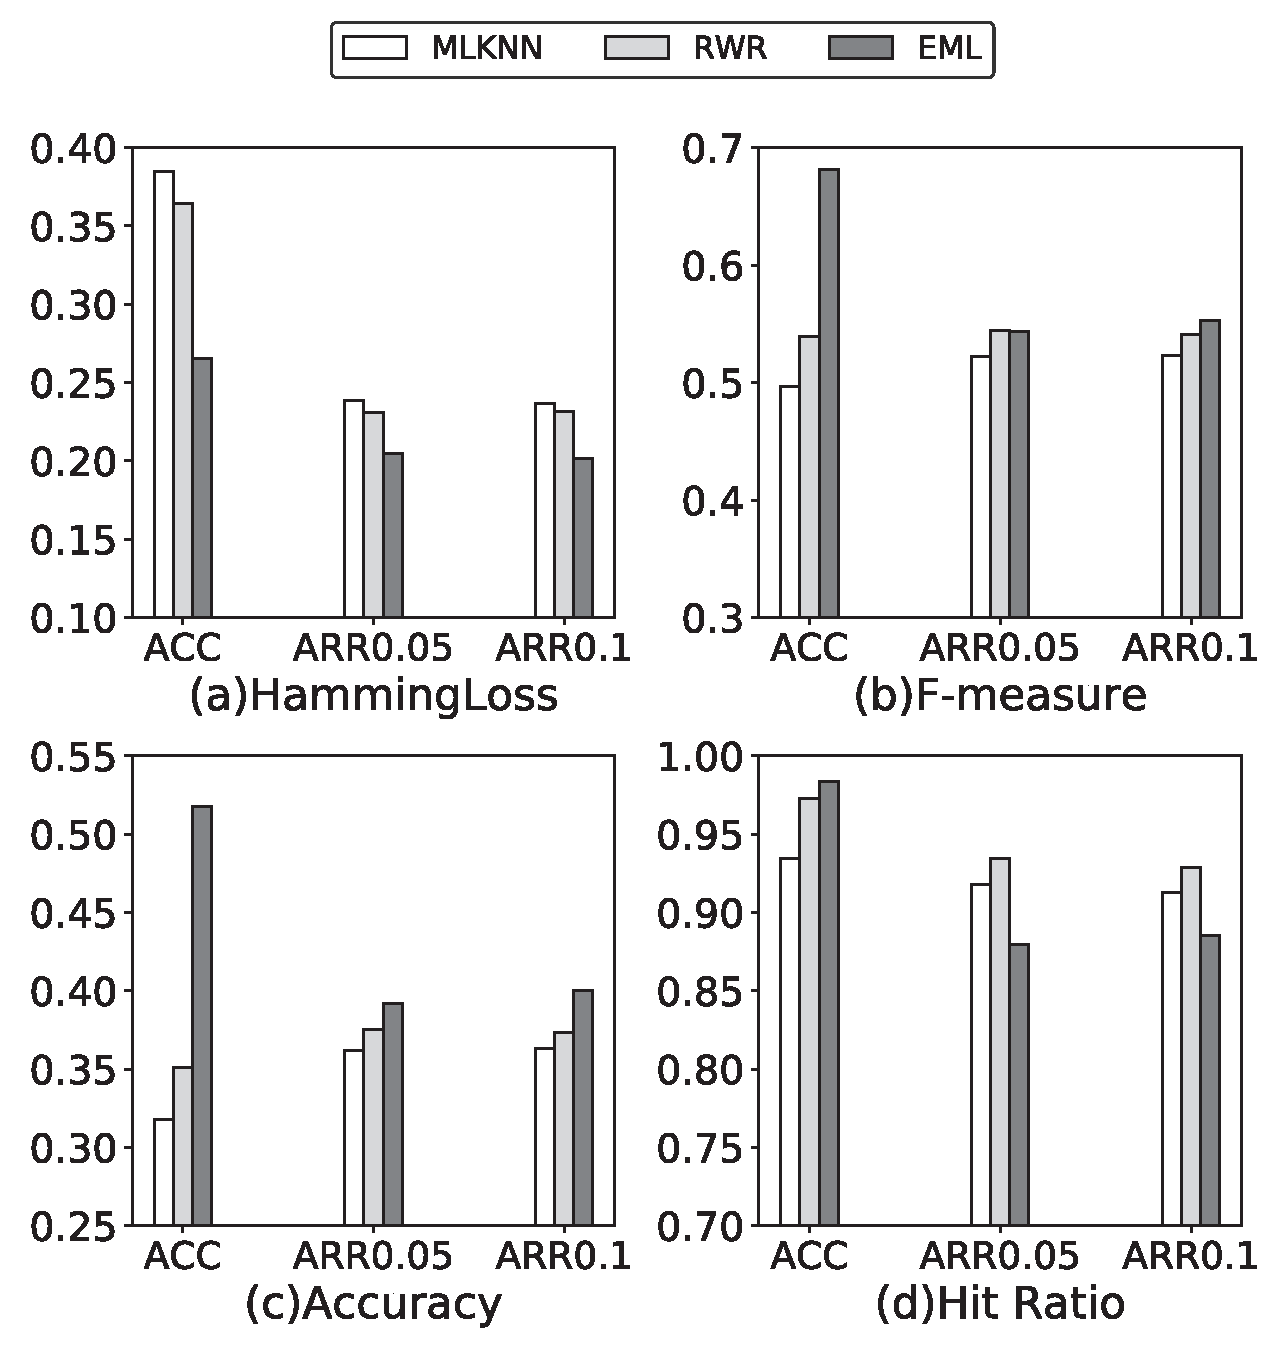
\includegraphics[width=6cm, height=5.5cm]{ML_SLP_EML.eps}}
	\caption{Comparison on \emph{Hamming Loss}, \emph{F-Measure}, \emph{Accuracy} and \emph{Hit Ratio} between \emph{MLKNN} based, \emph{RWR} based and \emph{EML} recommendation methods}
	\label{fig:slp_emlknn}
	%\normalsize
\end{figure}

1) Comparison on \emph{Hamming Loss}

The performance measure \emph{Hamming Loss} indicates how far the recommendation result is from the set of really appropriate algorithms. The value of \emph{HammingLoss} is between 0 and 1, and the smaller the \emph{Hamming Loss}, the better the recommendation. 

Comparison results on \emph{Hamming Loss} is shown in subfigure(a) of Figure \ref{fig:slp_emlknn}. It shows the \emph{Hamming Loss} when evaluating candidate algorithms with $ACC$ (accuracy), $ARR_{0.05}$ and $ARR_{0.1}$ as evaluation metrics to find appropriate algorithms for the training dataset. In this subfigure, the horizontal axis shows the evaluation metrics. The vertical axis shows the \emph{Hamming Loss} values of different recommendation methods, distinguished by bars of different colors. 

From subfigure(a), we can observe that: for all the three evaluation metrics, the \emph{Hamming Loss} values of \emph{EML} are much smaller than those of the three \emph{SLP} methods. In addition, the \emph{Hamming Loss} values has largest decrease in term of  $ACC$.

2) Comparison on \emph{F-Measure}

\emph{F-Measure} is a balance between \emph{Precision} and \emph{Recall}. Its value is between 0 and 1. Different from \emph{Hamming Loss}, the greater the value of \emph{F-Measure}, the better the recommendation. 

The comparison results on \emph{F-Measure} is shown in the second subfigure of Figure \ref{fig:slp_emlknn}. We can see from subfigure(b) that: among all the three recommendation methods, \emph{EML} acts the best, especially in $ACC$, which is about 1.5 times of the values of the \emph{ML-KNN} based methods. In $ARR_{0.05}$ and $ARR_{0.1}$, there is few difference among all three recommendation methods.

3) Comparison on \emph{Accuracy}

Subfigure(c) of Figure \ref{fig:slp_emlknn} depicts the recommendation performance comparison results among \emph{ML-KNN} based method, \emph{SLP} and \emph{EML} in terms of \emph{Accuracy}.

From this subfigure, we can observe that the comparison results in terms of \emph{Accuracy} are similar to those in terms of  \emph{F-Measure}. That is, \emph{Accuracy} of \emph{EML} is much greater than those of another two recommendation methods in $ACC$ and reaches 52\%, but has small increase in other evaluation metrics. 

4) Comparison on \emph{Hit Ratio}

\emph{Hit Ratio} reflects the probability that the recommended algorithms are appropriate for the given dataset. The greater the \emph{Hit Ratio}, the better the recommendation.

Comparison results on \emph{Hit Ratio} is shown in subfigure(d) of Figure \ref{fig:slp_emlknn}. We can observe from subfigure(d):
\begin{itemize}
	\item The maximum value of \emph{Hit Ratio} of \emph{EML} reaches 98\% in $ACC$ and is better than other two baseline methods.
	
	\item Compared in $ARR_{0.05}$ and $ARR_{0.1}$, the \emph{Hit Ratio} of \emph{EML} is smaller than those of the two baseline methods. Nevertheless, the values of \emph{Hit Ratio} of \emph{EML} are all larger than 87\%.
\end{itemize}

In $ARR_{0.05}$ and $ARR_{0.1}$, the actual total number of appropriate algorithms on 183 problems is 840 and 845 respectively. The recommended algorithm number of \emph{EML} is 765 and 770, which is smaller than the baseline methods, whose recommended number is certain and set to 5 for each classification problem, totally 915 on 183 historical problems. Thus, the comparison results on \emph{Hit Ratio} could be accepted.


\subsubsection{ Significance test for comparison between \emph{EML} and the baseline methods}

From the above analysis, we can conclude that \emph{EML} basically improves the \emph{ML-KNN} based and \emph{RWR} based methods on average. In this section, to verify the statistical significance of the improvements, we use the Wilcoxon signed-rank test, which is suggested by Demsar \upcite{Demsar2006Statistical} when comparing two methods on multiple problems, to compare \emph{EML} with other two baseline methods at significance level 0.05, respectively. %However, it's worth nothing that the Hit Ratio metric is an average value over all the test items so it is meaningless to do the statistical test on it.

\begin{table}[!h]
	\renewcommand\arraystretch{1.15}
	\centering
	\scriptsize
	\caption{Significance test result of comparison between \emph{ML-KNN} based, \emph{RWR} based and \emph{EML} recommendation methods}
	\label{table:statistical test}
	%			\begin{minipage}{0.5\linewidth}
	\scalebox{0.93}{
		\subtable[Statistical test result between \emph{ML-KNN} based and \emph{EML} methods]{
			\label{table:ML-KNN}
			\begin{tabular}{l|lccc}
				\hline
				Alternative & \multirow{2}{*}{Performance measures} & \multicolumn{3}{c}{Evaluation Metric} \\
				Hypothesis&  & ACC & $ARR_{0.05}$ & $ARR_{0.1}$ \\ \hline
				\multirow{5}{*}{\emph{EML} \textgreater \emph{ML-KNN}} 
				& Hamming Loss & 1.00 & 1.00 & 1.00  \\
				& F-Measure    & \textbf{0.00} & 0.27 & 0.10  \\
				& Accuracy     & \textbf{0.00} & 0.08 & \textbf{0.02}  \\
				& Hit Ratio    & \textbf{0.01} & 0.97 & 0.94  \\
				\cline{1-5}
				\multirow{5}{*}{\emph{EML} \textless \emph{ML-KNN}} 
				& Hamming Loss & \textbf{0.00} & \textbf{0.00} & \textbf{0.00}  \\
				& F-Measure    & 1.00 & 0.73 & 0.90  \\
				& Accuracy     & 1.00 & 0.92 & 0.98  \\
				& Hit Ratio    & 0.99 & \textbf{0.04} & 0.07  \\
				\cline{1-5}
				\specialrule{0em}{1pt}{1pt}
				& Win/Draw/Loss & 4/0/0 & 1/2/1 & 2/2/0 \\ 
				\hline
			\end{tabular}
		}
	}
	%			\end{minipage}			
	%			\begin{minipage}{0.48\linewidth}
	\scalebox{1.0}{
		\subtable[Statistical test result between \emph{RWR} based and \emph{EML} methods]{
			\label{table:RWR}
			\begin{tabular}{l|lccc}
				\hline
				Alternative & \multirow{2}{*}{Performance measures} & \multicolumn{3}{c}{Evaluation Metric} \\
				Hypothesis&  & ACC & $ARR_{0.05}$ & $ARR_{0.1}$ \\ \hline
				\multirow{5}{*}{\emph{EML} \textgreater \emph{RWR}} 
				& Hamming Loss & 1.00 & 1.00 & 1.00  \\
				& F-Measure    & \textbf{0.00} & 0.71 & 0.40  \\
				& Accuracy     & \textbf{0.00} & 0.37 & 0.13  \\
				& Hit Ratio    & 0.26 & 0.99 & 0.98  \\
				\cline{1-5}
				\multirow{5}{*}{\emph{EML} \textless \emph{RWR}} 
				& Hamming Loss & \textbf{0.00} & \textbf{0.00} & \textbf{0.00}  \\
				& F-Measure    & 1.00 & 0.29 & 0.60  \\
				& Accuracy     & 1.00 & 0.63 & 0.87  \\
				& Hit Ratio    & 0.78 & \textbf{0.01} & \textbf{0.02}  \\
				\cline{1-5}
				\specialrule{0em}{1pt}{1pt}
				& Win/Draw/Loss & 3/1/0 & 1/2/1 & 1/2/1 \\ 
				\hline
			\end{tabular}
		}
	}	
	
\end{table}

The statistical test results are shown in Table \ref{table:statistical test}, where each subtable contains two statistical test results. One's alternative hypothesis is that the evaluation values of \emph{EML} are statistically larger than the baseline method on each of the four recommendation performance measures in terms of each of the three evaluation metrics, while other's alternative hypothesis is on contrast.

In the table, a p-value < 0.05, which is presented by bold face, indicates that the alternative hypothesis is valid. For example, in subtable \ref{table:ML-KNN},  "\emph{EML} \textgreater \emph{ML-KNN}" indicates that the alternative hypothesis is that the evaluation values of \emph{EML} is statistically larger than the \emph{ML-KNN} based method. In ACC, when compared on \emph{F-Measure}, the statistical test value is 0.00, which is less that 0.05 and means that the alternative hypothesis is valid. For \emph{F-Measure}, the larger the value, the better the method (Note that \emph{Hamming Loss} is opposite). So \emph{EML} is statistically better than the \emph{ML-KNN} based method on F-Measure. 

Furthermore, we use the "Win/Draw/Loss" record to indicate the number of cases where \emph{EML} is statistically better than/equal to/worse than the compared method. Subtable \ref{table:ML-KNN} describes the statistical test results between the \emph{ML-KNN} based method and \emph{EML}, Subtable \ref{table:RWR} displays the test results between the\emph{RWR} based method and \emph{EML}.

From Table \ref{table:statistical test}, we can find that: In ACC, \emph{EML} acts statistically better than tow baseline methods on \emph{Hamming Loss}, \emph{F-Measure}, \emph{Accuracy} and \emph{Hit Ratio}. In $ARR_{0.05}$ or $ARR_{0.1}$, the performance of \emph{EML} is approximately equal to the \emph{RWR} based method but better than the \emph{ML-KNN} based method. Thus, we can conclude that the improvement of \emph{EML} to the baseline methods is statistically obvious.

\subsection{The comparison on the number of recommended algorithm}
\label{comparison on the number}

This section presents the result of comparison among baseline methods and \emph{EML} on the number of recommended algorithms. Since \emph{RWR} and \emph{ML-KNN} based methods identically recommend a certain number of algorithms for a given classification problem, \emph{RWR} based method is chosen as a representative to compare with \emph{EML}, which can automatically recommend the proper number of algorithms. The number of recommended algorithms of \emph{RWR} based method is set to 5 as its proposed paper suggests.

\begin{table}[!h]
	\renewcommand\arraystretch{1.15}
	\centering
	\caption{The comparison on the recommended algorithm number between \emph{RWR} based and \emph{EML} methods}
	\label{table:comparison on the number}
	\scalebox{1.2}{
		\scriptsize
		\begin{tabular}{lccc}
			\hline
			\multirow{2}{*}{Evaluation Metric} & \multicolumn{3}{c}{Win/Draw/Loss} \\
			& Win & Draw & Loss \\ \hline
			%\multirow{3}{*}{\emph{EML} \textgreater \emph{RWR}} 
			ACC             & 94 & 28 & 61  \\
			$ARR_{0.05}$    & 83 & 37 & 63  \\
			$ARR_{0.1}$     & 84 & 40 & 59  \\
			\hline
		\end{tabular}
	}	
	
\end{table} 

Table \ref{table:comparison on the number} shows the "Win/Draw/Loss" result of the comparison on 183 historical classification problems. The squared error between the recommended number and the actual number is used as a measure to judge which method's recommended algorithm number is closer to the actual number. And the "Win/Draw/Loss" record indicates the squared error of \emph{EML} is smaller than/equal to/larger than the compared method. 

From Table \ref{table:comparison on the number}, we can find that: No matter ACC, $ARR_{0.05}$ or $ARR_{0.1}$ is used, the recommended algorithm number of \emph{EML} is closer to the actual number. The difference in ACC is largest, correspondingly, the performance of \emph{EML} is far better than two baseline methods in ACC. In some way, the above results prove that the proposed \emph{EML} can automatically recommend the proper number of algorithms for different classification problems.


\section{Threats to Validity}
\label{threats}

A possible threat to validity of the work lies in whether the 183 datasets and the 20 candidate classification algorithms used in the empirical study are representative of the broader population of datasets and classification algorithms. Preferring to choose the widely used datasets and well known classification algorithms is the primary means by which this study tries to avoid sample bias.

Another threat is the use of \emph{Accuracy} and \emph{ARR} as the classification evaluation metrics. These two metrics have also been used in the baseline methods of this paper.

\section{Conclusion}	
\label{conclusion}

In this paper, we propose a two-layer classification algorithm recommendation method, \emph{EML}, which is based on ensemble learning. The proposed \emph{EML} method can take advantage of multiple different kinds of combinations of meta features and can automatically recommend different number of appropriate algorithm(s) for different classification problems.

Firstly, different kinds of combinations of meta features are generated to construct different Tier-1 learners. Then the Tier-2 training datasets corresponding to different labels are generated by Tier-1 learners and at last, the Tier-2 models are constructed over Tier-2 training datasets and used to recommend appropriate algorithm(s) for a new classification problem. 

In order to analyze the performance of \emph{EML}, 183 datasets, 20 classification algorithms were used to conduct an empirical study. The experimental results show that \emph{EML} is statistically better than the single link prediction based methods and the \emph{ML-KNN} based method. Moreover, we found that the recommended algorithm number of \emph{EML} is closer to the actual number than the baseline methods.

For the future work, we plan to focus on further improving the efficiency and quality of \emph{EML}. We will start from two points. One is to change the distance metrics of \emph{ML-KNN} when searching neighbours. The other is to use better meta feature and select useful combinations of meta features that are not only effective for classifying the Tier-2 training dataset but also fast.

\section*{References}

%\bibliography{mybibfile}

\begin{thebibliography}{10}
	\expandafter\ifx\csname url\endcsname\relax
	\def\url#1{\texttt{#1}}\fi
	\expandafter\ifx\csname urlprefix\endcsname\relax\def\urlprefix{URL }\fi
	\expandafter\ifx\csname href\endcsname\relax
	\def\href#1#2{#2} \def\path#1{#1}\fi
	
	\bibitem{quinlan1979discovering}
	J.~R. Quinlan, Discovering rules by induction from large collections of
	example, Expert Systems in the Micro Electronics Age.
	
	\bibitem{Quinlan1993Programs}
	J.~R. Quinlan, C4. 5: programs for machine learning, Elsevier, 2014.
	
	\bibitem{breiman1984classification}
	L.~Breiman, J.~Friedman, C.~J. Stone, R.~A. Olshen, Classification and
	regression trees, CRC press, 1984.
	
	\bibitem{Moore2005Internet}
	A.~W. Moore, D.~Zuev, Internet traffic classification using bayesian analysis
	techniques, in: ACM SIGMETRICS Performance Evaluation Review, Vol.~33, ACM,
	2005, pp. 50--60.
	
	\bibitem{webb2005not}
	G.~I. Webb, J.~R. Boughton, Z.~Wang, Not so naive bayes: aggregating
	one-dependence estimators, Machine learning 58~(1) (2005) 5--24.
	
	\bibitem{holte1993very}
	R.~C. Holte, Very simple classification rules perform well on most commonly
	used datasets, Machine learning 11~(1) (1993) 63--90.
	
	\bibitem{Cohen1995Fast}
	W.~W. Cohen, Fast effective rule induction, in: Proceedings of the twelfth
	international conference on machine learning, 1995, pp. 115--123.
	
	\bibitem{Wolpert2002The}
	D.~H. Wolpert, The supervised learning no-free-lunch theorems, in: World
	Conference on Soft Computing, 2002, pp. 25--42.
	
	\bibitem{Ali2006On}
	S.~Ali, K.~A. Smith, On learning algorithm selection for classification,
	Applied Soft Computing 6~(2) (2006) 119--138.
	
	\bibitem{Brazdil2000A}
	P.~B. Brazdil, C.~Soares, A comparison of ranking methods for classification
	algorithm selection, in: European Conference on Machine Learning, 2000, pp.
	63--74.
	
	\bibitem{song2012automatic}
	Q.~Song, G.~Wang, C.~Wang, Automatic recommendation of classification
	algorithms based on data set characteristics, Pattern recognition 45~(7)
	(2012) 2672--2689.
	
	\bibitem{Chekina2012Meta}
	L.~Chekina, L.~Rokach, B.~Shapira, Meta-learning for selecting a multi-label
	classification algorithm, in: IEEE International Conference on Data Mining
	Workshops, 2012, pp. 220--227.
	
	\bibitem{Smith2009Cross}
	K.~A. Smith-Miles, Cross-disciplinary perspectives on meta-learning for
	algorithm selection, ACM Computing Surveys (CSUR) 41~(1) (2009) 6.
	
	\bibitem{Brazdil:2008:MAD:1507541}
	P.~Brazdil, C.~G. Carrier, C.~Soares, R.~Vilalta, Metalearning: Applications to
	data mining, Springer Science \& Business Media, 2008.
	
	\bibitem{Aha1992Generalizing}
	D.~W. Aha, Generalizing from case studies: A case study, in: Proc. of the 9th
	International Conference on Machine Learning, 1992, pp. 1--10.
	
	\bibitem{Wang2015An}
	G.~Wang, Q.~Song, X.~Zhu, An improved data characterization method and its
	application in classification algorithm recommendation, Applied Intelligence
	43~(4) (2015) 892--912.
	
	\bibitem{Roy2017Meta}
	A.~Roy, R.~M.~O. Cruz, R.~Sabourin, G.~D.~C. Cavalcanti, Meta-regression based
	pool size prediction scheme for dynamic selection of classifiers, in:
	International Conference on Pattern Recognition, 2017.
	
	\bibitem{Smith2001Modelling}
	K.~A. Smith, F.~Woo, V.~Ciesielski, R.~Ibrahim, Modelling the relationship
	between problem characteristics and data mining algorithm performance using
	neural networks, in: C. dagli, et al, in: Eds.), Smart Engineering System
	Design: Neural Networks, Fuzzy Logic, Evolutionary Programming, Data Mining,
	and Complex Systems, Citeseer, 2001.
	
	\bibitem{Smith2002Matching}
	K.~A. Smith, F.~Woo, V.~Ciesielski, R.~Ibrahim, Matching data mining algorithm
	suitability to data characteristics using a self-organizing map, Springer,
	2002, pp. 169--179.
	
	\bibitem{Kalousis2004On}
	A.~Kalousis, J.~Gama, M.~Hilario, On data and algorithms: Understanding
	inductive performance, Machine learning 54~(3) (2004) 275--312.
	
	\bibitem{Gore2013Dynamic}
	S.~Gore, N.~Pise, Dynamic algorithm selection for data mining classification,
	International Journal of Scientific and Engineering Research 4~(12) (2013)
	2029--2033.
	
	\bibitem{Ali2017Accurate}
	R.~Ali, S.~Lee, T.~C. Chung, Accurate multi-criteria decision making
	methodology for recommending machine learning algorithm, Expert Systems with
	Applications 71 (2017) 257--278.
	
	\bibitem{Brazdil1994Characterizing}
	P.~Brazdil, J.~Gama, B.~Henery, Characterizing the applicability of
	classification algorithms using meta-level learning, in: European conference
	on machine learning, Springer, 1994, pp. 83--102.
	
	\bibitem{Gama1995Characterization}
	J.~Gama, P.~Brazdil, Characterization of classification algorithms, Progress in
	Artificial Intelligence (1995) 189--200.
	
	\bibitem{Brazdil2003Ranking}
	P.~B. Brazdil, C.~Soares, J.~P. Da~Costa, Ranking learning algorithms: Using
	ibl and meta-learning on accuracy and time results, Machine Learning 50~(3)
	(2003) 251--277.
	
	\bibitem{Lee2013Automatic}
	J.~W. Lee, C.~Giraud-Carrier, Automatic selection of classification learning
	algorithms for data mining practitioners, Intelligent Data Analysis 17~(4)
	(2013) 665--678.
	
	\bibitem{Bensusan2001Estimating}
	H.~Bensusan, A.~Kalousis, Estimating the predictive accuracy of a classifier,
	Machine Learning: ECML 2001 (2001) 25--36.
	
	\bibitem{Reif2014Automatic}
	M.~Reif, F.~Shafait, M.~Goldstein, T.~Breuel, A.~Dengel, Automatic classifier
	selection for non-experts, Pattern Analysis and Applications 17~(1) (2014)
	83--96.
	
	\bibitem{Balte2015Algorithm}
	A.~Balte, N.~Pise, R.~Agrawal, Algorithm selection based on landmarking
	meta-feature, Communications on Applied Electronics 2~(6) (2015) 23--27.
	
	\bibitem{Wang2014A}
	G.~Wang, Q.~Song, X.~Zhang, K.~Zhang, A generic multilabel learning-based
	classification algorithm recommendation method, ACM Transactions on Knowledge
	Discovery from Data (TKDD) 9~(1) (2014) 7.
	
	\bibitem{Zhang2007A}
	M.-L. Zhang, Z.-H. Zhou, Ml-knn: A lazy learning approach to multi-label
	learning, Pattern Recognition 40~(7) (2007) 2038 -- 2048.
	
	\bibitem{Zhu2018A}
	X.~Zhu, X.~Yang, c.~Ying, g.~Wang, A new classification algorithm
	recommendation method based on link prediction, Knowledge Based Systems
	xx~(xx) (2018) xxxx.
	\newblock \href
	{http://dx.doi.org/https://doi.org/10.1016/j.knosys.2018.07.015}
	{\path{doi:https://doi.org/10.1016/j.knosys.2018.07.015}}.
	
	\bibitem{Breiman1996Stacked}
	L.~Breiman, Stacked regressions, Machine Learning 24~(1) (1996) 49--64.
	
	\bibitem{Brodley1993Addressing}
	C.~E. Brodley, Addressing the selective superiority problem: Automatic
	algorithm/model class selection, in: Proceedings of the tenth international
	conference on machine learning, 1993, pp. 17--24.
	
	\bibitem{Balte2014Meta}
	A.~Balte, N.~Pise, P.~Kulkarni, Meta-learning with landmarking: A survey,
	International Journal of Computer Applications 105~(8) (2014) 47--51.
	
	\bibitem{Kalousis1999NOEMON}
	A.~Kalousis, T.~Theoharis, Noemon: Design, implementation and performance
	results of an intelligent assistant for classifier selection, Intelligent
	Data Analysis 3~(5) (1999) 319--337.
	
	\bibitem{Sohn1999Meta}
	S.~Y. Sohn, Meta analysis of classification algorithms for pattern recognition,
	IEEE Transactions on Pattern Analysis and Machine Intelligence 21~(11) (1999)
	1137--1144.
	
	\bibitem{Ali2018A}
	R.~Ali, A.~M. Khatak, F.~Chow, S.~Lee, A case-based meta-learning and reasoning
	framework for classifiers selection, in: Proceedings of the 12th
	International Conference on Ubiquitous Information Management and
	Communication, IMCOM '18, ACM, New York, NY, USA, 2018, pp. 31:1--31:6.
	
	\bibitem{Bensusan1998God}
	H.~Bensusan, God doesn't always shave with occam's razor-learning when and how
	to prune, Machine Learning: ECML-98 (1998) 119--124.
	
	\bibitem{Peng2002Improved}
	Y.~Peng, P.~A. Flach, C.~Soares, P.~Brazdil, Improved dataset characterisation
	for meta-learning, in: International Conference on Discovery Science,
	Springer, 2002, pp. 141--152.
	
	\bibitem{Pfahringer2000Meta}
	B.~Pfahringer, H.~Bensusan, C.~G. Giraud-Carrier, Meta-learning by landmarking
	various learning algorithms, in: Seventeenth International Conference on
	Machine Learning, 2000, pp. 743--750.
	
	\bibitem{Bensusan2000Casa}
	H.~Bensusan, C.~Giraud-Carrier, Casa batlo is in passeig de gracia or
	landmarking the expertise space, University of Bristol, 2000.
	
	\bibitem{Ho2000Complexity}
	T.~Ho, Complexity of classification problems and comparative advantages of
	combined classifiers, Multiple Classifier Systems (2000) 97--106.
	
	\bibitem{Ho2002Complexity}
	T.~K. Ho, M.~Basu, Complexity measures of supervised classification problems,
	IEEE transactions on pattern analysis and machine intelligence 24~(3) (2002)
	289--300.
	
	\bibitem{Elizondo2009Estimation}
	D.~A. Elizondo, R.~Birkenhead, M.~Gamez, N.~Garcia, E.~Alfaro, Estimation of
	classification complexity, in: Neural Networks, 2009. IJCNN 2009.
	International Joint Conference on, IEEE, 2009, pp. 764--770.
	
	\bibitem{Kasture2015Dynamic}
	R.~Kasture, A.~Kher, S.~Shetty, P.~Jain, N.~Pise, A.~Pate, Dynamic ranking of
	classification algorithms, Multidisciplinary Journal of Research in
	Engineering and Technology (2015) 8--14.
	
	\bibitem{Pise2016Algorithm}
	N.~Pise, P.~Kulkarni, Algorithm selection for classification problems, in: Sai
	Computing Conference, 2016, pp. 203--211.
	
	\bibitem{Yang2017Choosing}
	Z.~Yang, H.~Li, S.~Ali, Y.~Ao, Choosing classification algorithms and its
	optimum parameters based on data set characteristics, Journal of Computers
	28~(5) (2017) 26--38.
	
	\bibitem{dietterich2002ensemble}
	T.~G. Dietterich, et~al., Ensemble learning, The handbook of brain theory and
	neural networks 2 (2002) 110--125.
	
	\bibitem{hansen1990neural}
	L.~K. Hansen, P.~Salamon, Neural network ensembles, IEEE Transactions on
	Pattern Analysis \& Machine Intelligence~(10) (1990) 993--1001.
	
	\bibitem{Toothaker1993Multiple}
	L.~E. Toothaker, Multiple comparisons for researchers, Sage Publications, Inc,
	1991.
	
	\bibitem{Demsar2006Statistical}
	J.~Demšar, Statistical comparisons of classifiers over multiple data sets,
	Journal of Machine learning research 7~(Jan) (2006) 1--30.
	
	\bibitem{Hall1999Correlation}
	M.~Hall, Correlation-based feature selection for machine learning, PhD Thesis,
	Waikato Univer-sity 19.
	
	\bibitem{korf1993linear}
	R.~E. Korf, Linear-space best-first search, Artificial Intelligence 62~(1)
	(1993) 41--78.
	
	\bibitem{Freund1995A}
	Y.~Freund, R.~E. Schapire, A desicion-theoretic generalization of on-line
	learning and an application to boosting, Springer Berlin Heidelberg, 1995.
	
	\bibitem{Dua2019UCI}
	D.~Dua, C.~Graff, \href{http://archive.ics.uci.edu/ml}{{UCI} machine learning
		repository} (2017).
	\newline\urlprefix\url{http://archive.ics.uci.edu/ml}
	
	\bibitem{Pantelis2005}
	P.~Vlachos, Statlib---datasets archive, \url{http://lib.stat.cmu.edu/datasets/}
	(Jul. 2005).
	
	\bibitem{OpenMLR2017}
	G.~Casalicchio, J.~Bossek, M.~Lang, D.~Kirchhoff, P.~Kerschke, B.~Hofner,
	H.~Seibold, J.~Vanschoren, B.~Bischl,
	\href{http://doi.acm.org/10.1007/s00180-017-0742-2}{Openml: An r package to
		connect to the machine learning platform openml}, Computational Statistics
	32~(3) (2017) 1--15.
	\newblock \href {http://dx.doi.org/10.1007/s00180-017-0742-2}
	{\path{doi:10.1007/s00180-017-0742-2}}.
	\newline\urlprefix\url{http://doi.acm.org/10.1007/s00180-017-0742-2}
	
	\bibitem{alcala2011keel}
	J.~Alcal{\'a}-Fdez, A.~Fern{\'a}ndez, J.~Luengo, J.~Derrac, S.~Garc{\'\i}a,
	L.~S{\'a}nchez, F.~Herrera, Keel data-mining software tool: data set
	repository, integration of algorithms and experimental analysis framework.,
	Journal of Multiple-Valued Logic \& Soft Computing 17.
	
	\bibitem{liu2010link}
	W.~Liu, L.~L{\"u}, Link prediction based on local random walk, EPL (Europhysics
	Letters) 89~(5) (2010) 58007.
	
	\bibitem{Kearns1997Algorithmic}
	M.~Kearns, D.~Ron, Algorithmic stability and sanity-check bounds for
	leave-one-out cross-validation, Neural Computation 11~(6) (1997) 1427--1453.
	
\end{thebibliography}


\end{document}